%!TEX program = xelatex
%!TEX root = ../all.tex

\chapter{Loss functions \& training}
\section*{Loss function}

The concept of a loss function lies at the very heart of machine learning. In its most general form, the loss function $\mathcal{L}:\mathcal{Y}\times\mathcal{Y}\mapsto\Real$ serves as a quantitative measure of the \alert{cost} incurred when we refer to a predicted value $y$ instead of the true target value $t$ for any subsequent decision or action. Here, both $y$ and $t$ are elements belonging to the target space $\mathcal{Y}$, which could represent real numbers in regression problems, discrete class labels in classification tasks, or more complex structured outputs in other learning scenarios.

\medskip

To understand why we need such a measure, consider that in supervised learning our goal is not merely to generate predictions, but to generate \emph{good} predictions—ones that closely align with the true underlying relationship between inputs and outputs. The loss function provides precisely this measure of quality. Specifically, it quantifies how well the prediction function $h$ performs on a given input-output pair. For an input $\x$ with corresponding true output $y$, we evaluate the quality of our prediction through: 
	\begin{myequation}
	\mathcal{R}(\x, y)=L(h(\x), y)
	\end{myequation}

This individual loss tells us how far off we are for a single prediction, but in practice we work with entire datasets. Therefore, the loss function becomes a fundamental component of what we call the \alert{empirical risk}, which aggregates the loss across all examples in our training set. The empirical risk is defined as the average value of the loss function applied to all predicted value-target value pairs in the training set $\mathcal{T}$:
\begin{myequation}
	\mathcal{\overline R}_{\mathcal{T}}(h)=\frac{1}{|\mathcal{T}|}\sum_{(x,t)\in\mathcal{T}}L(h(x),t)
\end{myequation}

This quantity serves as our primary indicator of model quality, at least with respect to the available training data. It answers the question: "On average, how much error does our prediction function make?" The lower this value, the better our model fits the training data. However, we must always keep in mind that minimizing empirical risk on training data is not our ultimate goal—we truly care about performance on unseen data, which relates to the concept of generalization.

\medskip

During the training phase, our objective is to minimize the empirical risk with respect to the prediction function $h$. In practice, this means we work with parametric functions $h=h_{\theta}$, where the behavior of $h$ is completely determined by a set of parameters $\Vtheta = (\theta_0, \theta_1, \ldots, \theta_d)$. The training process can thus be viewed as a search through parameter space for the configuration that yields the smallest empirical risk.

This minimization problem can be equivalently formulated as minimizing the overall loss:
\begin{myequation}
\mathcal{L}(\Vtheta;\mathcal{T})=\sum_{i=1}^nL_i(\Vtheta)
\end{myequation} 
which represents the sum of individual loss functions $L_i=L(\Vtheta; \x_i,t_i)$ computed for each data point $(\x_i, t_i)$ in our training set. The notation emphasizes that the loss depends on both the parameters $\Vtheta$ and the specific training example being considered.


\subsection*{Loss function minimization approaches}

Having defined what we want to minimize, we now face the crucial question: how can we actually tackle the problem of minimizing the loss function in practice? This is not merely a theoretical concern—the efficiency and effectiveness of our optimization strategy directly determines whether we can successfully train our models.

Ideally, our goal is to find a \alert{global minimum} of the loss function, which would represent the best possible set of parameters for our model across the entire parameter space. A global minimum is a point where the loss is lower than at any other point in the parameter space, meaning we have found the truly optimal configuration.

\medskip

One classical approach to finding minima relies on fundamental results from calculus. The key insight is that at any minimum (whether local or global), the gradient—that is, the vector of all partial derivatives—must equal zero. This is because if the gradient were non-zero at some point, we could move in the direction opposite to the gradient and further decrease the function value, contradicting the assumption that we are at a minimum.

Mathematically, we seek to solve:
\begin{myequation}
\nabla\mathcal{L}(\Vtheta;\mathcal{T})=\Zero
\end{myequation}

Let us clarify the notation here. The symbol $\nabla$ denotes the gradient operator, which, given a multivariate function $f(x_1,\ldots,x_m)$, returns the vector of its partial derivatives with respect to each variable:
\begin{myequation}
\nabla f=\vcol{\frac{\partial f}{\partial x_1}}{\frac{\partial f}{\partial x_m}}
\end{myequation}

An important geometric interpretation helps build intuition: the gradient at any given point $\overline{x}_1,\ldots,\overline{x}_m$ in the domain space of $f$ is a vector pointing in the direction of steepest ascent from that point. Conversely, the negative of the gradient points in the direction of steepest descent—a fact we will exploit later.

Setting the gradient to $\Zero$ means solving a system of equations where each component is set to zero:
\begin{myequation}
\frac{\partial}{\partial\theta_i}\mathcal{L}(\Vtheta;\mathcal{T})=0\hspace{.5cm}\forall i
\end{myequation}

Each equation in this system represents the condition that the loss function does not increase (to first order) when we make an infinitesimal change to parameter $\theta_i$ while holding all other parameters fixed. Finding values of $\Vtheta$ that satisfy all these equations simultaneously would give us candidate points where the loss could be minimal.

\medskip

However, this elegant mathematical approach faces several significant practical challenges that limit its applicability, especially in modern machine learning contexts. First and foremost, this system of equations typically has multiple solutions. These solutions include not only local minima (which are our desired outcomes) but also local maxima (which are the worst possible points to stop at) and saddle points (which are neither minima nor maxima but rather inflection points that are critical nonetheless). Without additional analysis, we cannot distinguish between these different types of critical points.

Moreover, and perhaps more critically, in many practical cases—especially those involving complex models like neural networks—solving these equations analytically is either extremely difficult or outright impossible. The loss functions we encounter in deep learning are highly non-linear, involving compositions of many non-linear activation functions, and analytical solutions simply do not exist in closed form. This necessitates the use of numerical optimization methods.


\subsection*{Gradient descent}

Given the challenges of analytical approaches, we turn to iterative numerical methods that can approximate solutions. Among these, \alert{gradient descent} stands out as one of the most fundamental and widely used algorithms in machine learning. While it may not guarantee finding the global minimum, it provides a practical and computationally efficient way to find a local minimum of the empirical risk function $\mathcal{\overline R}_{\mathcal{T}}(\Vtheta)$.

The gradient descent algorithm follows a beautifully simple principle: if we want to minimize a function, we should move in the direction where the function decreases most rapidly. Since the gradient points in the direction of steepest ascent, moving in the opposite direction—that is, in the direction of the negative gradient—takes us toward steepest descent.

\medskip

The process begins by initializing our parameters at some starting point, which we denote as $\Vtheta^{(0)} = (\theta_{0}^{(0)}, \theta_{1}^{(0)}, \ldots, \theta_{d}^{(0)})$. This initialization is often random or based on some heuristic, and it comes with an initial error value given by:
\begin{myequation}
\mathcal{\overline R}_{\mathcal{T}}(\Vtheta^{(0)}).
\end{myequation}

This initial error tells us how poorly our randomly initialized model performs—typically quite poorly indeed! The goal of gradient descent is to iteratively improve upon this initial configuration.

The iterative procedure works by repeatedly modifying the current parameter values $\Vtheta^{(i-1)}$ in the direction of \alert{steepest descent} of the empirical risk function $\mathcal{\overline R}_{\mathcal{T}}(\Vtheta)$. Specifically, this means moving in the opposite direction of the gradient of the empirical risk evaluated at our current position $\Vtheta^{(i-1)}$. We take a step down the slope of the error surface, moving toward (we hope) a valley where the error is minimized.

At each iteration $i$ of the algorithm, each parameter $\theta_{j}^{(i-1)}$ is updated according to the following rule:
\begin{myequation}
\theta_j^{(i)} := \theta_j^{(i-1)} - \eta \frac{\partial}{\partial \theta_j }\mathcal{\overline R}_{\mathcal{T}}(\Vtheta)\Big|_{\Vtheta^{(i-1)}} =
\theta_j^{(i-1)} - \frac{\eta}{|\mathcal{T}|}\sum_{(\x, t)\in\mathcal{T}} \frac{\partial}{\partial \theta_j} L(h_{\Vtheta}(\x), t)\Big|_{\Vtheta^{(i-1)}},
\end{myequation}

Let us unpack this equation carefully, as it encodes the entire essence of gradient descent. The parameter $\eta$ is called the \alert{learning rate}, and it controls the step size during each update. Think of it as determining how aggressive we are in following the gradient's direction: a large learning rate means we take big steps, potentially converging faster but risking overshooting the minimum; a small learning rate means we take tiny steps, converging more reliably but possibly very slowly. The partial derivative term tells us the direction and rate of change of the loss with respect to this particular parameter, and the negative sign ensures we move downhill rather than uphill.

In matrix form, which provides a more compact notation, this update rule can be written as:
\begin{myequation}
\Vtheta^{(i)} := \Vtheta^{(i-1)} - \eta \;\nabla\mathcal{\overline R}_{\mathcal{T}}(\Vtheta)\Big|_{\Vtheta^{(i-1)}} = 
\Vtheta^{(i-1)} - \frac{\eta}{|\mathcal{T}|}\sum_{(\x,t)\in\mathcal{T}} \nabla L(h_{\Vtheta}(\x), t)\Big|_{\Vtheta^{(i-1)}}.
\end{myequation}

This formulation makes clear that we update all parameters simultaneously based on the full gradient vector computed from all training examples.

\medskip

While this method allows us to approximate a local minimum in a computationally tractable manner, the outcome depends heavily on several factors, particularly the initial parameter values chosen. The loss landscape in high-dimensional parameter spaces can be extraordinarily complex, with many valleys, peaks, and plateaus. Different starting points can lead us to entirely different local minima, some of which may be much better than others.

This observation leads us to several key challenges and questions that practitioners must grapple with:
\begin{itemize}
\item We are fundamentally interested in finding a global minimum—the absolute best configuration of parameters—but gradient descent can easily get stuck at local minima. How can we encourage exploration of the parameter space to avoid settling for poor local optima?

\item How do we handle saddle points, which are critical points (where the gradient is zero) that are neither minima nor maxima? In high-dimensional spaces, saddle points are actually far more common than local minima, and gradient descent can slow down dramatically near these points, even though they are not minima at all.

\item How quickly does the method converge, and what factors influence its speed? The convergence rate depends on the learning rate, the conditioning of the loss function (how stretched or round the error surface is), and the quality of our initialization.

\item What happens if the learning rate is too large or too small? Can we adapt it during training to achieve better performance?
\end{itemize}

These challenges make the minimization process considerably more complex than it might initially appear, but gradient descent and its many variants remain among the most widely used methods in practice for parameter optimization. Modern deep learning has developed numerous sophisticated extensions—including momentum methods, adaptive learning rates, and second-order approximations—that address many of these challenges while maintaining computational efficiency.


\subsection*{Convexity}

Having explored the challenges of optimization, we now turn to a mathematical property that, when present, dramatically simplifies our task: convexity. Understanding convexity is crucial because it tells us when optimization becomes significantly easier—when we can be confident that any local minimum we find is actually the global minimum.

Let us begin with the geometric definition. A set of points $S\subset\Real^d$ is said to be \alert{convex} if and only if for any two points $\x_1,\x_2\in S$ and any scalar $\lambda\in (0,1)$, we have:
\begin{myequation}
\lambda\x_1+(1-\lambda)\x_2\in S
\end{myequation}

In intuitive terms, this means that if we take any two points in the set and draw a straight line segment connecting them, every point on that line segment must also belong to the set. Convex sets have no "holes" or "indentations"—they are, in a sense, solid and without concavities.

\begin{figure}[ht]
\begin{center}
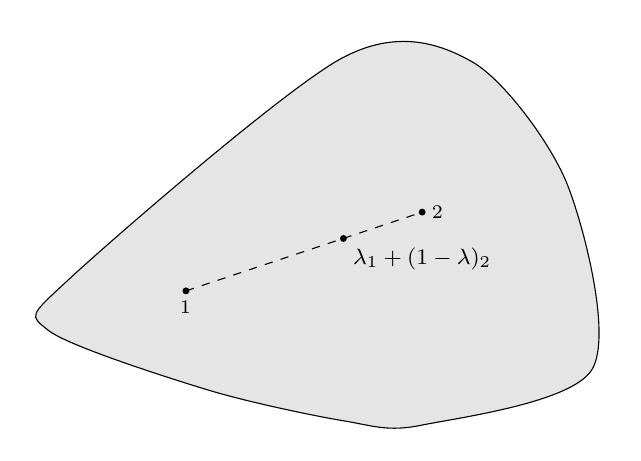
\begin{tikzpicture}[scale=.5]
\draw [fill=gray!20] plot [mark=none, smooth cycle] coordinates {(-6.5,4) (-2.5,2.5) (1,1.7) (3,1.591) (7.312,3) (6.7,7.668) (4.264,10.821) (0.948,10.904) (-5.973,5.294)};
\coordinate (g) at (3,7);
\fill (g) circle (2.5pt) node [right] {$\x_2$};
\coordinate (p) at (-3,5);
\fill (p) circle (2.5pt) node [below] {$\x_1$};
\draw [dashed] (p) --  (g);
\coordinate (e) at (1,6.33);
\fill (e) circle (2.5pt) node [below right] {\footnotesize $\lambda \x_1+(1-\lambda)\x_2$};
\end{tikzpicture}
\end{center}
\caption{Convex set}
\end{figure}

\medskip

Now, extending this concept from sets to functions, we say that a function $f(\x)$ is \alert{convex} if and only if the set of points lying on or above the graph of the function forms a convex set. More precisely, for all points $\x_1,\x_2$ in the domain and all $\lambda\in (0,1)$, the following inequality must hold:
\begin{myequation}
f(\lambda\x_1+(1-\lambda)\x_2)\leq \lambda f(\x_1)+(1-\lambda) f(\x_2)
\end{myequation}

This elegant condition has a beautiful geometric interpretation: if we take any two points on the graph of $f$ and connect them with a straight line segment, that line segment must lie on or above the graph of the function. In other words, the function never curves upward more than a straight line would—it has no concave regions where it dips down.

\begin{figure}[ht]
\begin{center}
\begin{tikzpicture}[scale=1.3]
\node at (0,4.2) [anchor=north east] {$f(t_1)$};
\node at (2.4,0) [anchor=north east] {$t_1$};
\node at (0,1.3) [anchor=north east] { $f(t_2)$};
\node at (0,1.9) [anchor=north east] { $f(\lambda t_1+(1-\lambda)t_2)$};
\node at (5.2,0) [anchor=north east] { $t_2$};
\node at (4.6,0) [anchor=north east] { $\lambda t_1+(1-\lambda)t_2$};

\node at (0,3.1) [anchor=north east] { $\lambda f(t_1)+(1-\lambda)f(t_2)$};
\node at (6.5,2) [anchor=north east] { $f(x)$};
\begin{axis}[
axis x line=bottom,
axis y line=left,
ticks=none,
xmin=-3, xmax=2, ymin=-.5, ymax=3.5]
\addplot [xkcdCerise, thick, domain=-2:1, samples=201]{x^2};
\addplot [xkcdSlateBlue, thick, domain=-2.5:1, samples=201]{-x+.75};
\addplot[samples=50, smooth,black] coordinates {(-1.5,-4.5)(-1.5, 2.25)};
\addplot[samples=50, smooth,black] coordinates {(-3,2.25)(-1.5,2.25)};
\addplot[samples=50, smooth,black] coordinates {(.5,-4.5)(.5,.25)};
\addplot[samples=50, smooth,black] coordinates {(-3,.25)(.5,.25)};
\addplot[samples=50, smooth,dashed] coordinates {(-.788,-4.5)(-.788,1.5)};
\addplot[samples=50, smooth,black, dashed] coordinates {(-3,.622)(-.788,.622)};
\addplot[samples=50, smooth,black, dashed] coordinates {(-3,1.538)(-.788,1.538)};
\end{axis}
\end{tikzpicture}
\end{center}
\caption{Convex function}
\end{figure}

An even stronger property is \alert{strict convexity}, where the inequality becomes strict. A function $f(\x)$ is strictly convex if and only if for all distinct points $\x_1\neq\x_2$ and all $\lambda\in (0,1)$, we have:
\begin{myequation}
f(\lambda\x_1+(1-\lambda)\x_2)< \lambda f(\x_1)+(1-\lambda) f(\x_2)
\end{myequation}

The difference between convexity and strict convexity is subtle but important: strictly convex functions curve strictly upward—they cannot have any flat regions or linear segments.

\medskip

Why does convexity matter so profoundly for optimization? The answer lies in a remarkable theoretical result: \emph{if $f(\x)$ is a convex function, then any local minimum of $f$ is also a global minimum}. This means that if we use gradient descent and it converges to a local minimum (where the gradient is zero), we can be confident that we have found the best possible solution. There are no hidden valleys elsewhere in the parameter space with lower function values.

The situation is even better for strictly convex functions: if $f$ is \alert{strictly convex}, there exists \emph{only one} local minimum for $f$, and it is necessarily the global minimum. This uniqueness property is extraordinarily powerful—it means that regardless of where we initialize gradient descent, we will always converge to the same optimal solution (assuming appropriate learning rates and sufficient iterations).

Therefore, when our loss function $\mathcal{L}(\Vtheta;\mathcal{T})$ is convex, solving the system of equations:
\begin{myequation}
    \nabla\mathcal{L}(\Vtheta;\mathcal{T})=\Zero
\end{myequation}
is guaranteed to provide us with a global minimum, making the optimization problem tractable both theoretically and practically.

\medskip

A particularly important special case occurs when $f(\x)$ is a quadratic function—that is, when it can be written as a second-degree polynomial in the variables. Quadratic functions are always convex (and strictly convex if their matrix of second derivatives is positive definite), and they admit closed-form solutions. This favorable situation arises in several classical machine learning models, including linear regression with squared error loss and certain formulations of logistic regression.

Unfortunately, this convenient property does not hold for more complex models, particularly neural networks with non-linear activation functions. The loss surface of a deep neural network is highly non-convex, with potentially many local minima, saddle points, and plateaus. This non-convexity is one reason why training deep networks remains challenging and why much research focuses on developing better optimization algorithms and initialization strategies.

\medskip

To leverage convexity when possible, we can exploit some useful mathematical properties. Let us recall two fundamental results about convex functions:
\begin{enumerate}
\item The sum of (strictly) convex functions is itself (strictly) convex. This is straightforward to verify: if $f$ and $g$ are both convex, then their sum $h = f + g$ satisfies the convexity inequality because both $f$ and $g$ individually satisfy it.

\item The product of a (strictly) convex function and a positive constant is (strictly) convex. Scaling preserves the geometric property of curving upward.
\end{enumerate}

These properties have immediate implications for our empirical risk. Recall that:
\begin{myequation}
	\mathcal{\overline R}_{\mathcal{T}}(h)=\frac{1}{|\mathcal{T}|}\sum_{(\x,t)\in\mathcal{T}}L(h(\x),t)\propto\sum_{(\x,t)\in\mathcal{T}}L(\Vtheta; \x,t)
\end{myequation}

The empirical risk is simply a scaled sum of individual loss terms evaluated at each training example. Applying the properties above, we can draw several important conclusions:
\begin{itemize}
\item If each individual loss function $L(\Vtheta; \x,t)$ is (strictly) convex with respect to the parameters $\Vtheta$, then the overall empirical risk is also (strictly) convex. This follows immediately from the fact that we are forming a weighted sum (with positive weights) of convex functions.

\item If $L(\Vtheta; \x,t)$ is convex, then any local minimum of the empirical risk is guaranteed to be a global minimum. This means gradient descent, if it converges, will find the optimal solution regardless of initialization.

\item If $L(\Vtheta; \x,t)$ is strictly convex, then there exists a unique minimum of the empirical risk. Not only is any local minimum global, but there is exactly one such minimum. This provides maximal certainty in our optimization procedure.
\end{itemize}

These results highlight why much effort in machine learning theory and practice goes into designing loss functions and model architectures that preserve convexity, or at least approximate it sufficiently well. When convexity can be achieved or approximated, optimization becomes vastly more reliable and predictable, allowing us to focus on other aspects of model design and deployment.



\section*{Some common loss functions}

Having established the theoretical framework for loss functions and their optimization, we now turn our attention to the practical question: what specific loss functions should we use in different machine learning scenarios? The choice of loss function is not merely a technical detail—it profoundly influences both the optimization landscape we must navigate and the type of solution our model will ultimately learn. Different loss functions encode different assumptions about what constitutes a "good" prediction and how severely we should penalize different types of errors.

In this section, we examine the most commonly used loss functions in supervised learning, organized by the type of learning task they are designed for. We begin with regression problems, where we predict continuous values, and then move to classification problems, where we assign discrete labels.

\subsection*{Loss functions for regression}

Let us first consider the case of \alert{regression}, where our goal is to predict a continuous numerical output. The regression setting has several defining characteristics that shape our choice of loss function:

\begin{itemize}
\item Both the true target value $t$ and our prediction $h(\x)$ are real-valued numbers, typically in $\Real$ or some bounded subset thereof. This means we are working in a continuous output space rather than with discrete categories.

\item The natural notion of error in this setting relates to some form of distance measure between points in this continuous space. We want to quantify "how far" our prediction is from the truth, and different distance measures lead to different loss functions with distinct properties.
\end{itemize}

The choice of distance measure is not arbitrary—it reflects our assumptions about the nature of errors and their consequences. Should large errors be penalized much more severely than small ones? Should we treat positive and negative errors symmetrically? These considerations guide our selection of an appropriate loss function.

\subsubsection*{Quadratic loss}

The most ubiquitous and widely used loss function for regression tasks is the \alert{quadratic loss}, also known as squared error or $L_2$ loss. It is defined simply as:
\begin{myequation}
L(y,t)=(y-t)^2
\end{myequation} 

This deceptively simple formula has profound implications. The quadratic loss measures the squared Euclidean distance between prediction and target, meaning that errors are penalized quadratically—an error twice as large incurs four times the loss. This has the effect of making the optimization procedure particularly sensitive to outliers, as we shall discuss.

\begin{figure}[ht]
\begin{center}
\begin{tikzpicture}[scale=1]
\node at (3.6,0) [anchor=north east] {\footnotesize $t$};
\begin{axis}[
legend style={
at={(1.5,1)},
anchor=north east,
draw=none,
fill=none},
ytick={0},
yticklabels={$0$},
xticklabels={,,}, 
axis x line=bottom,
axis y line=left,
xlabel={$y$},
x label style={at={(axis description cs:0.99,0)},anchor=north},
%ticks=none,
xmin=-2, xmax=2, ymin=-1.1, ymax=3.5]

\addplot [xkcdCerise, thick, domain=-2:2, samples=201]{x^2};
\addplot [xkcdSlateBlue, thick, domain=-2:2, samples=201]{2*x};
\addplot[samples=50, thick, smooth,black, dotted] coordinates {(-3,0)(3,0)};
\legend{loss,loss gradient}
\end{axis}
\end{tikzpicture}
\end{center}
\caption{Quadratic loss function and its gradient. Note the parabolic shape and the linear gradient.}
\end{figure}

\medskip

When we apply quadratic loss across our entire training set, we obtain the empirical risk in a particularly elegant form:
\begin{myequation}
	\mathcal{\overline R}_{\mathcal{T}}(h)=\frac{1}{|\mathcal{T}|}\sum_{(\x,t)\in\mathcal{T}}(h(\x)-t)^2
\end{myequation}

This quantity, often called the \alert{mean squared error} (MSE), represents the average squared deviation between our predictions and the true values across all training examples. Minimizing this quantity is equivalent to finding the prediction function that best fits the training data in the least-squares sense.

\medskip

In the particularly common case of \alert{linear regression}, where we assume the underlying relationship between inputs and outputs is linear, the prediction is performed by means of a linear function $h(\x)=\w^T\x+b$, where $\w$ represents a weight vector and $b$ is a bias term. Substituting this into our empirical risk formula results in an overall loss function to be minimized:
\begin{myequation}
	\mathcal{L}(\w,b;\mathcal{T})=\sum_{(\x,t)\in\mathcal{T}}(\w^T\x+b-t)^2
\end{myequation}

This formulation has several extraordinarily favorable mathematical properties that make it the workhorse of classical statistical learning:

\begin{itemize}
\item Since the quadratic function is strictly convex, the overall loss $\mathcal{L}(\w,b;\mathcal{T})$ has only one local minimum, which is necessarily the global minimum. This guarantees that any optimization procedure that successfully finds a local minimum has found the best possible solution.

\item The gradient of the loss with respect to the parameters is linear, which makes optimization particularly tractable. Specifically, we can compute:
\begin{myequation}
\frac{\partial}{\partial w_i}\mathcal{L}(\w,b;\mathcal{T})=\sum_{(\x,t)\in\mathcal{T}}(\w^T\x+b-t)x_i\hspace{1cm}
\frac{\partial}{\partial b}\mathcal{L}(\w,b;\mathcal{T})=\sum_{(\x,t)\in\mathcal{T}}(\w^T\x+b-t)
\end{myequation}

where $x_i$ denotes the $i$-th component of the input vector $\x$. The linearity of these gradients means that gradient descent will converge smoothly without oscillations or instabilities.

\item In fact, for linear regression with quadratic loss, we can even derive a closed-form analytical solution by setting these gradients to zero and solving the resulting system of linear equations. This is the famous \alert{normal equations} approach, which provides an exact solution without requiring iterative optimization.
\end{itemize}

Despite these attractive properties, quadratic loss is not without its drawbacks. Its primary weakness is that it is not robust to outliers. Because errors are squared, a single data point with a very large error can dominate the overall loss, causing the fitted model to be pulled dramatically toward that outlier at the expense of fitting the bulk of the data well. This sensitivity can be problematic in real-world datasets where outliers or measurement errors are common.

\subsubsection*{Absolute loss}

While quadratic loss is mathematically convenient and has elegant properties, its lack of robustness to outliers motivates the search for alternatives. One natural alternative is the \alert{absolute loss}, also known as $L_1$ loss or mean absolute error:
\begin{myequation}
L(y,t)=|y-t|
\end{myequation}

The absolute loss measures the absolute value of the difference between prediction and target, penalizing errors linearly rather than quadratically. This seemingly small change has significant practical consequences: whereas quadratic loss penalizes an error of magnitude $\epsilon$ with cost $\epsilon^2$, absolute loss penalizes it with cost $\epsilon$. This means that large errors grow linearly rather than quadratically, making absolute loss much more robust to outliers.

\begin{figure}[ht]
\begin{center}
\begin{tikzpicture}[scale=1]
\node at (3.6,0) [anchor=north east] { $t$};
\begin{axis}[
legend style={
at={(1.5,1)},
anchor=north east,
draw=none,
fill=none},
ytick={-1,0,1},
yticklabels={ $-1$, $0$, $1$},
xticklabels={,,}, 
axis x line=bottom,
axis y line=left,
xlabel={$y$},
x label style={at={(axis description cs:0.99,0)},anchor=north},
%ticks=none,
xmin=-2, xmax=2, ymin=-1.1, ymax=3.5]
\addplot [xkcdCerise, thick, domain=-2:0, samples=201]{-x};
\addplot [xkcdSlateBlue, thick, domain=0:2, samples=201]{1};
\addplot [xkcdCerise, thick, domain=0:2, samples=201]{x};
\addplot [xkcdSlateBlue, thick, domain=-2:0, samples=201]{-1};
\addplot[samples=50, thick, smooth,black, dotted] coordinates {(-3,0)(3,0)};
\addplot[samples=50, thick, smooth,black, dotted] coordinates {(-3,1)(3,1)};
\addplot[samples=50, thick, smooth,black, dotted] coordinates {(-3,-1)(3,-1)};
\legend{loss,loss gradient}
\end{axis}
\end{tikzpicture}
\end{center}
\caption{Absolute loss function and its gradient. The V-shape is characteristic, with constant gradient magnitude.}
\end{figure}

An important feature of absolute loss is immediately apparent from examining its gradient: the gradient is piecewise constant, taking the value $-1$ when $y < t$ and $+1$ when $y > t$. This constant gradient magnitude means that gradient descent will take steps of uniform size regardless of how far the current prediction is from the target (modulo the learning rate). This is in stark contrast to quadratic loss, where the gradient grows linearly with the error, causing larger steps when predictions are far from targets.

The absolute loss is convex, which ensures that any local minimum is global, but it is not strictly convex (notice the flat gradient regions). This means there may be multiple optimal solutions, though in practice this rarely causes difficulties. A more significant practical challenge is that the gradient is undefined at $y = t$, where the function has a sharp corner. However, this can be handled using subgradient methods, which we will discuss in more detail when examining classification losses.

\subsubsection*{Huber loss}

Given the trade-offs between quadratic and absolute loss—the former being smooth and easy to optimize but sensitive to outliers, the latter being robust but having discontinuous derivatives—a natural question arises: can we design a loss function that combines the best of both worlds? The \alert{Huber loss} provides exactly such a compromise.

The Huber loss is quadratic for small errors (like quadratic loss) but transitions to linear growth for large errors (like absolute loss). This hybrid behavior is achieved through the following piecewise definition:

\begin{myequation}
L(t,y)=
\begin{cases}
\frac{1}{2}(t-y)^2 & |t-y|\leq\delta \\
\delta(|t-y|-\frac{\delta}{2}) & |t-y|>\delta
\end{cases}
\end{myequation}

The parameter $\delta$ controls the transition point between quadratic and linear behavior. For errors smaller than $\delta$ in magnitude, the loss behaves quadratically, providing smooth gradients that facilitate efficient optimization. For errors larger than $\delta$, the loss grows linearly, providing robustness against outliers by preventing them from dominating the overall loss.

\begin{figure}[ht]
\begin{center}
\begin{tikzpicture}[scale=1]
\node at (3.6,0) [anchor=north east] { $t$};
\begin{axis}[
legend style={
at={(1.5,1)},
anchor=north east,
draw=none,
fill=none},
ytick={-1,0,1},
yticklabels={ $-\delta$, $0$, $\delta$},
xticklabels={,,}, 
axis x line=bottom,
axis y line=left,
xlabel={$y$},
x label style={at={(axis description cs:0.99,0)},anchor=north},
%ticks=none,
xmin=-2, xmax=2, ymin=-1.1, ymax=3.5]
\addplot [xkcdCerise, thick, domain=-1:1, samples=201]{x^2/2};
\addplot [xkcdSlateBlue, thick, domain=-1:1, samples=201]{x};
\addplot [xkcdCerise, thick, domain=-2:-1, samples=201]{-x-1/2};
\addplot [xkcdCerise, thick, domain=1:2, samples=201]{x-1/2};
\addplot [xkcdSlateBlue, thick, domain=-3:-1, samples=201]{-1};
\addplot [xkcdSlateBlue, thick, domain=1:3, samples=201]{1};
\addplot[samples=50, thick, smooth,black, dotted] coordinates {(-3,0)(3,0)};
\addplot[samples=50, thick, smooth,black, dotted] coordinates {(-3,1)(3,1)};
\addplot[samples=50, thick, smooth,black, dotted] coordinates {(-3,-1)(3,-1)};
\legend{loss,loss gradient}
\end{axis}
\end{tikzpicture}
\end{center}
\caption{Huber loss combines quadratic behavior near zero with linear growth for large errors.}
\end{figure}

The Huber loss represents an elegant compromise that is particularly valuable in practical applications where we expect our data to contain some outliers but still want to benefit from the smooth optimization properties of quadratic loss for the majority of well-behaved data points. The choice of $\delta$ becomes a hyperparameter that can be tuned based on the expected scale and frequency of outliers in the specific application domain.

\subsection*{Loss functions for classification}

We now shift our attention from regression to classification, where the prediction task is fundamentally different in nature. In classification, we assign inputs to discrete categories or classes rather than predicting continuous values. This discrete structure necessitates a different approach to measuring error and, consequently, different loss functions.

There are essentially two distinct approaches to classification, which lead to different types of loss functions:

\begin{itemize}
\item \textbf{Direct class prediction}: The prediction function returns a specific class label directly. In this case, we measure error based on the coincidence (or lack thereof) between the predicted class and the true class.

\item \textbf{Probabilistic prediction}: The prediction function returns a probability distribution over the set of possible classes. Here, we measure error based on the cumulative difference between the predicted probability distribution and the true distribution (which assigns probability 1 to the correct class and 0 to all others).
\end{itemize}

These two approaches imply fundamentally different definitions of what constitutes an error:
\begin{itemize}
\item In the first case, we care only about whether the predicted class matches the real class—there is no notion of being "almost correct."
\item In the second case, we care about the confidence of predictions—a prediction that assigns high probability to the correct class is better than one that barely favors it, even if both make the same final classification decision.
\end{itemize}

For concreteness and clarity, we will focus on the \alert{binary classification} case, where there are exactly two classes. We identify these classes with target values $t \in \{-1, +1\}$, a convention that proves mathematically convenient. The extension to multi-class classification follows similar principles but with added notational complexity.

In what follows, we will assume that our classifier produces a real-valued output $y = h(\x)$, which can be interpreted as a confidence score. The sign of $y$ determines the predicted class ($+1$ if $y > 0$, $-1$ if $y < 0$), while the magnitude $|y|$ represents the confidence of that prediction. This framework, where a single real number encodes both the predicted class and the prediction confidence, is extremely common and underlies many important classification algorithms.

\subsubsection*{0/1 loss}

The most intuitive and "natural" loss function for classification problems is the \alert{0/1 loss}, which directly encodes the notion of correctness: we incur a loss of 1 for an incorrect prediction and a loss of 0 for a correct prediction. Formally:

\begin{myequation}
L(t,y)=
\begin{cases}
1 &\text{sgn}(y)\not= t \\
0 &\text{sgn}(y)= t
\end{cases}
\end{myequation}

where $\text{sgn}(y)$ denotes the sign of $y$, defined as $+1$ if $y>0$ and $-1$ if $y \leq 0$.

Using our convention where predictions are real numbers $y$ and targets are in $\{-1, +1\}$, we can express this more compactly. Observe that $ty < 0$ precisely when the signs of $t$ and $y$ differ—that is, when we have made an incorrect prediction. Thus, we can write:
\begin{myequation}
L(t,y) = {\large\mathds{1}}[t y< 0]
\end{myequation}
where ${\large\mathds{1}}[\cdot]$ is the indicator function, equal to 1 when its argument is true and 0 otherwise.

\begin{figure}[ht]
\begin{center}
\begin{tikzpicture}[scale=1]
\node at (3.6,0) [anchor=north east] { $0$};
\begin{axis}[
ytick={0,1},
yticklabels={ $0$,  $1$},
xticklabels={,,}, 
%yticklabels={,,}, 
axis x line=bottom,
axis y line=left,
xlabel={$ty$},
x label style={at={(axis description cs:0.99,0)},anchor=north},
%ticks=none,
xmin=-2, xmax=2, ymin=-.1, ymax=3.5]
\addplot [xkcdCerise, thick, domain=-2:0, samples=201]{1};
\addplot [xkcdCerise, thick, domain=0:2, samples=201]{0};
\end{axis}
\end{tikzpicture}
\end{center}
\caption{The 0/1 loss is a step function that assigns uniform cost to all errors.}
\end{figure}

The 0/1 loss has obvious intuitive appeal—it directly measures classification accuracy, which is often what we ultimately care about. When we minimize the empirical risk under 0/1 loss, we are explicitly minimizing the classification error rate on our training data. However, despite this conceptual clarity, using 0/1 loss in practice is highly problematic for several fundamental reasons:

\begin{itemize}
\item \textbf{Non-convexity}: The 0/1 loss is not convex. This means that our loss landscape may have many local minima, and gradient-based optimization methods offer no guarantee of finding the global minimum. Worse, different initializations may lead to vastly different solutions.

\item \textbf{Non-smoothness}: The function is not smooth—it has a discontinuous jump at $ty = 0$. The first derivative is undefined at this point, making it impossible to apply standard calculus-based optimization techniques.

\item \textbf{Zero gradients almost everywhere}: Perhaps most critically, the gradient of 0/1 loss is zero almost everywhere (specifically, everywhere except at $ty = 0$, where it is undefined). This means gradient descent cannot make any progress—the gradient provides no information about which direction to move in parameter space to reduce the loss.

\item \textbf{Computational intractability}: If we assume a linear prediction function $y = \w^T\x+b$, the empirical risk becomes:
\begin{myequation}
 \mathcal{\overline R}_{\mathcal{T}}(h)=\frac{1}{|\mathcal{T}|}\sum_{(\x,t)\in\mathcal{T}}{\large\mathds{1}}[(\w^T\x+b) t< 0]
\end{myequation}

The problem of finding the values $\w, b$ that minimize the overall number of classification errors is NP-hard. This means that, unless P=NP (which is widely believed to be false), there exists no polynomial-time algorithm guaranteed to find the optimal solution. The problem remains computationally intractable even for moderately sized datasets.
\end{itemize}

These severe limitations make direct optimization of 0/1 loss impractical for most real-world applications. This fundamental difficulty motivates the development of alternative loss functions that approximate 0/1 loss but possess better mathematical properties.

\subsubsection*{Convex surrogate loss functions}

Given the intractability of directly optimizing 0/1 loss, a central question in classification theory is: what alternative loss functions can we use that are both mathematically tractable and still produce good classifiers? The answer lies in \alert{convex surrogate loss functions}, which have become the foundation of modern classification algorithms.

A surrogate loss function is one that serves as a substitute for 0/1 loss during optimization. For a surrogate to be useful, it should satisfy several key properties:

\begin{itemize}
\item \textbf{Upper bound property}: The surrogate should approximate 0/1 loss \alert{from above}, meaning that the surrogate loss is always at least as large as the 0/1 loss. This ensures that minimizing the surrogate will also tend to minimize the actual classification error. Formally, for all $t$ and $y$, we require:
\begin{myequation}
L_{\text{surrogate}}(t,y) \geq {\large\mathds{1}}[ty < 0]
\end{myequation}

\item \textbf{Convexity}: The surrogate should be convex with respect to the prediction $y$ (and consequently with respect to the model parameters). This guarantees that any local minimum we find is also a global minimum, making optimization reliable and predictable.

\item \textbf{Smoothness}: The surrogate should be smooth, with well-defined derivatives almost everywhere. This allows us to use gradient-based optimization methods effectively, with gradients that provide meaningful information about which direction to move in parameter space.
\end{itemize}

Different surrogate loss functions make different trade-offs in how they approximate 0/1 loss. A key distinction among them lies in the relevance or weight they assign to different types of errors. Some surrogates penalize all errors equally, while others heavily penalize certain types of errors (such as very confident but incorrect predictions) while being more lenient toward others (such as correct predictions with low confidence).

In what follows, we examine the most important and widely used surrogate loss functions, analyzing their properties and understanding when each is most appropriate.

\subsubsection*{Perceptron loss}

The \alert{perceptron loss} provides one of the simplest modifications to 0/1 loss. Recall that 0/1 loss assigns the same cost of 1 to every misclassified example, regardless of how wrong the prediction is. The perceptron loss refines this by taking into account the magnitude of the error.

The key insight is the following: if we assume our prediction $y$ is a real value, then for a misclassified element (where $ty < 0$), we can measure the severity of the error using the value $-ty$. This quantity is positive for misclassified examples and increases as the prediction becomes more confidently wrong. The perceptron loss is defined as:
\begin{myequation}
L(t,y)=\max{}(0, -ty)
\end{myequation}

Let us unpack what this means:
\begin{itemize} 
\item For correctly classified elements where $ty > 0$, the loss is zero. The perceptron loss does not penalize correct predictions at all, regardless of how confident they are.

\item For incorrectly classified elements where $ty < 0$, the loss equals $-ty = |ty|$, which is the absolute magnitude of the product $ty$. The more negative this product (meaning the more confident the wrong prediction), the higher the penalty.
\end{itemize}

The main philosophical difference from 0/1 loss is this: the perceptron loss distinguishes between different types of errors based on their severity. An example that is predicted to be strongly in class $+1$ (large positive $y$) when it actually belongs to class $-1$ (so $t = -1$) incurs a much larger loss than an example whose prediction is only slightly positive. This makes intuitive sense—we should care more about fixing egregious errors than marginal ones.

From a mathematical perspective, the perceptron loss has several important properties:
\begin{itemize}
\item It is continuous everywhere
\item Its gradient is continuous almost everywhere (specifically, everywhere except at $ty = 0$)
\item It is convex, ensuring that local minima are global
\item However, it is not strictly convex (it has linear regions)
\item Importantly, it is \textbf{not} a surrogate loss in the strict sense—it does not always upper bound the 0/1 loss. For correctly classified examples near the decision boundary, the perceptron loss is 0 while 0/1 loss is also 0, but the perceptron loss doesn't provide the same guarantee for all correctly classified points
\end{itemize}

\begin{center}
\begin{tikzpicture}[scale=1]
\node at (3.6,0) [anchor=north east] { $0$};
\begin{axis}[legend style={
at={(1.5,1)},
anchor=north east,
draw=none,
fill=none},
ytick={0,1},
yticklabels={ $0$, $1$},
xticklabels={,,}, 
axis x line=bottom,
axis y line=left,
xlabel={$ty$},
x label style={at={(axis description cs:0.99,0)},anchor=north},
xmin=-2, xmax=2, ymin=-.1, ymax=3.5]
\addplot [xkcdCerise, thick, domain=0:2, samples=201, line width=1pt]{0};
\addplot [xkcdTeal, thick, domain=-2:0, samples=201, line width=1pt]{1};
\addplot [xkcdCerise, thick, domain=-2:0, samples=201, line width=1pt]{-x};
\addplot [xkcdTeal, thick, domain=0:2, samples=201, line width=1pt]{0};
\addplot[samples=50, smooth,black, dotted] coordinates {(-3,0)(3,0)};
\addplot[samples=50, smooth,black, dotted] coordinates {(-3,1)(3,1)};
\addplot[samples=50, smooth,black, dotted] coordinates {(-3,-1)(3,-1)};
\legend{Perceptron loss, 0/1 loss}
\end{axis}
\end{tikzpicture}
\end{center}

The perceptron loss is historically significant as it underlies the classical perceptron algorithm, one of the earliest learning algorithms developed in the 1950s. While simple, it demonstrates the key principle of using a tractable surrogate to approximate the intractable 0/1 loss.

\subsubsection*{Hinge loss}

The \alert{hinge loss} represents a refinement of the perceptron loss and is the foundation of one of the most important classification algorithms: the Support Vector Machine (SVM). Like the perceptron loss, it is linear for misclassified examples, but it introduces a crucial modification: it also penalizes correctly classified examples that are too close to the decision boundary.

The hinge loss is defined as:
\begin{myequation}
L(t,y)=\max(0, 1-ty)
\end{myequation}

Compare this carefully to the perceptron loss $\max(0, -ty)$. The critical difference is the constant $1$ instead of $0$ inside the expression. This seemingly minor change has profound implications:

\begin{itemize} 
\item The loss is zero only when $ty \geq 1$, not merely when $ty > 0$. This means that correct predictions (where $ty > 0$) can still incur a penalty if they are not sufficiently confident.

\item For misclassified examples where $ty < 0$, the loss is $1 - ty$, which grows linearly as the prediction becomes more wrong.

\item For correctly classified examples where $0 < ty < 1$, the loss is $1 - ty > 0$. These are correct but "weak" predictions—the classifier has made the right choice but without much confidence. The hinge loss penalizes such weak correct predictions, encouraging the learner to push them further from the decision boundary.

\item Only when $ty \geq 1$ does the loss become zero. This means the classifier is encouraged to make confident correct predictions, with a "margin" of safety between the prediction and the decision threshold.
\end{itemize}

From a mathematical standpoint, hinge loss possesses several valuable properties:
\begin{itemize}
\item It is continuous everywhere
\item Its gradient is continuous almost everywhere (except at $ty = 1$, where it has a corner)
\item It is convex (though not strictly convex, due to the flat region where $ty > 1$)
\item Crucially, it is a proper surrogate loss—it provides an upper bound on 0/1 loss for all values of $ty$
\end{itemize}

\begin{center}
\begin{tikzpicture}[scale=1]
\node at (3.6,0) [anchor=north east] { $0$};
\node at (5.6,0) [anchor=north east] { $1$};
\begin{axis}[legend style={
at={(1.5,1)},
anchor=north east,
draw=none,
fill=none},
ytick={0,1},
yticklabels={ $0$, $1$},
xticklabels={,,}, 
axis x line=bottom,
axis y line=left,
xlabel={$ty$},
x label style={at={(axis description cs:0.99,0)},anchor=north},
xmin=-2, xmax=2, ymin=-.1, ymax=3.5]
\addplot [xkcdCerise, thick, domain=1:2, samples=201, line width=1pt]{0};
\addplot [xkcdTeal, thick, domain=-2:0, samples=201, line width=1pt]{1};
\addplot [xkcdCerise, thick, domain=-2:1, samples=201, line width=1pt]{1-x};
\addplot [xkcdTeal, thick, domain=0:2, samples=201, line width=1pt]{0};
\addplot[samples=50, smooth,black, dotted] coordinates {(-3,0)(3,0)};
\addplot[samples=50, smooth,black, dotted] coordinates {(-3,1)(3,1)};
\addplot[samples=50, smooth,black, dotted] coordinates {(-3,-1)(3,-1)};
\legend{Hinge loss, 0/1 loss}
\end{axis}

\end{tikzpicture}
\end{center}

The hinge loss is used in Support Vector Machine training, where the goal is not just to classify examples correctly but to find a decision boundary that maximizes the margin—the distance between the boundary and the nearest examples from each class. The penalty for weak correct predictions (where $0 < ty < 1$) is precisely what encourages this margin-maximizing behavior.

\medskip

\textbf{A technical note on differentiation}: The hinge loss $L_H(t,y)=\max(0,1-ty)$ is not differentiable with respect to $y$ at the point $ty=1$, where the function has a corner. Similarly, the perceptron loss has this issue at $ty=0$. At these points, the derivative is undefined in the classical sense.

For example, computing the derivative of hinge loss yields:
\begin{myequation}
\frac{\partial}{\partial y}L_H=\begin{cases}
-t\hspace{1cm}& ty<1\\
0\hspace{1cm}&ty>1\\
\text{undefined}&ty=1
\end{cases}
\end{myequation}

This non-differentiability poses a challenge if we want to apply gradient descent. However, we can work around this issue using the concept of a \alert{subgradient}.

\subsubsection*{Subgradients}

To understand subgradients, let us first recall what the gradient does for differentiable convex functions. Given a convex function $f$ and a point $x$ where $f$ is differentiable, the gradient $\nabla f|_x$ defines a linear function (specifically, the tangent hyperplane at $x$) that provides a lower bound for $f$ everywhere:

\begin{myequation}
f(x')\geq f(x)+\nabla f|_x \cdot (x'-x) \quad \text{for all } x'
\end{myequation}

This is a fundamental property of convex functions—the tangent line at any point lies below the function. Geometrically, this means that if we stand at point $x$ on the graph of $f$, the function never dips below the plane defined by the gradient at that point.

\medskip 

Now, what happens at a singular point $x$ where $f$ is not differentiable and the classical gradient $\nabla f|_x$ does not exist? The key insight is that we can generalize the notion of gradient by considering \emph{any} linear function that still provides a lower bound for $f$. We call such a function a \alert{subgradient}.

Formally, a subgradient $\overline{\nabla}f|_x$ at point $x$ is any vector satisfying:
\begin{myequation}
f(x')\geq f(x)+\overline{\nabla}f|_x \cdot (x'-x) \quad \text{for all } x'
\end{myequation}

The crucial difference is that at non-differentiable points, there may be multiple valid subgradients—indeed, there is typically an entire set of them. Any vector whose corresponding linear function stays below the graph of $f$ qualifies as a subgradient. At differentiable points, the subgradient coincides with the ordinary gradient, so this definition extends rather than contradicts the classical notion.

\medskip

For the hinge loss specifically, we can observe geometrically what the valid subgradients are. At the corner point $ty=1$, the function transitions from having slope $-t$ (when $ty < 1$) to having slope $0$ (when $ty > 1$). Any line whose slope lies between these two values—that is, any slope in the interval $[-t, 0]$ when $t=1$, or equivalently $[0, -t]$ when $t=-1$—will provide a valid lower bound and thus constitute a valid subgradient.

\begin{center}
\begin{tikzpicture}[scale=1]
\node at (4.2,0) [anchor=north east] { $0$};
%\node at (5.6,0) [anchor=north east] {\footnotesize $1$};
\begin{axis}[legend style={
at={(1.5,1)},
anchor=north east,
draw=none,
fill=none},
ytick={0,1},
yticklabels={ $0$, $1$},
xticklabels={,,}, 
axis x line=bottom,
axis y line=left,
xlabel={$ty$},
x label style={at={(axis description cs:0.99,0)},anchor=north},
xmin=-2, xmax=3, ymin=-.9, ymax=3.5]
\addplot [xkcdCerise, thick, domain=1:3, samples=201, line width=1pt]{0};
%\addplot [teal, domain=-2:0, samples=201, line width=1pt]{1};
\addplot [xkcdCerise, thick, domain=-2:1, samples=201, line width=1pt]{1-x};
\addplot [xkcdOrange, thick, domain=-2:3, samples=201, line width=.5pt, dashed]{.5-.5*x};
\addplot [xkcdDenimBlue, thick, domain=-2:3, samples=201, line width=.5pt, dashed]{.3-.3*x};
%\addplot [teal, domain=0:2, samples=201, line width=1pt]{0};
\addplot[samples=50, smooth,black, dotted] coordinates {(-3,0)(4,0)};
\addplot[samples=50, smooth,black, dotted] coordinates {(-3,1)(4,1)};
\addplot[samples=50, smooth,black, dotted] coordinates {(-3,-1)(4,-1)};
\end{axis}
\end{tikzpicture}
\end{center}

In practice, when implementing gradient descent with hinge loss, we typically choose a convenient subgradient from this range. A common choice is to use the horizontal line (slope $0$) as the subgradient at $ty=1$. This corresponds to assuming that $\frac{\partial L_H}{\partial y}=0$ at the singular point, which gives us:

\begin{myequation}
\overline{\nabla}_y L_H=\begin{cases}
-t\hspace{1cm}& ty<1\\
0\hspace{1cm}&ty\geq 1
\end{cases}
\end{myequation}

This subgradient can be used in place of the ordinary gradient in gradient descent algorithms, and the resulting optimization procedure is guaranteed to converge to a minimum (though possibly more slowly than with smooth functions). The use of subgradients extends the applicability of gradient-based methods to a much broader class of convex but non-smooth loss functions, making practical optimization feasible even when classical calculus-based methods would fail.

\subsubsection*{Square loss in classification}

Having examined loss functions specifically designed for classification, we might wonder: could we simply adapt regression losses to the classification setting? The \alert{squared loss for classification} does exactly this, modifying the quadratic loss we saw earlier to account for the structure of binary classification:

\begin{myequation}
L(t,y)=(1-ty)^2
\end{myequation}

Notice how this differs from the regression version $(t-y)^2$. Here, we penalize the squared difference between the desired quantity $ty = 1$ (which would indicate a correct and confident prediction) and the actual product $ty$ of target and prediction.

The squared loss for classification has some appealing mathematical properties:
\begin{itemize} 
\item It is continuous everywhere and infinitely differentiable—as smooth as a function can be
\item Its gradient is continuous and can be computed analytically everywhere
\item It is convex, ensuring unique global minima
\item Unlike hinge loss, there are no corners or non-differentiable points to worry about
\end{itemize}

However, these mathematical conveniences come with significant practical drawbacks:

\begin{itemize}
\item It is \textbf{not} a surrogate loss—it does not upper bound 0/1 loss everywhere. For correctly classified examples with $ty > 1$, the squared loss can be less than the 0/1 loss.

\item \textbf{Extreme errors are heavily penalized}: Because errors are squared, a prediction that is very wrong (large negative $ty$) incurs an enormous penalty that grows quadratically. This makes the loss extremely sensitive to outliers or mislabeled examples in the training data.

\item \textbf{Symmetric penalization around zero}: Even largely correct predictions with $ty \gg 1$ are penalized quadratically as $ty$ increases. This seems counterintuitive—we are punishing the classifier for being very confident in correct predictions! This symmetry is inherited from the regression setting where over-prediction and under-prediction are both undesirable, but in classification, high confidence in correct predictions should generally be encouraged, not penalized.
\end{itemize}

\begin{center}
\begin{tikzpicture}[scale=1]
\node at (3.6,0) [anchor=north east] { $0$};
\begin{axis}[legend style={
at={(1.5,1)},
anchor=north east,
draw=none,
fill=none},
ytick={0,1},
yticklabels={ $0$, $1$},
xticklabels={,,}, 
axis x line=bottom,
axis y line=left,
xlabel={$ty$},
x label style={at={(axis description cs:0.99,0)},anchor=north},
%ticks=none,
xmin=-2, xmax=2, ymin=-.1, ymax=3.5]

\addplot [xkcdCerise, thick, domain=-2:2, samples=201, line width=1pt]{(1-x)^2};
\addplot [xkcdTeal, thick, domain=-2:0, samples=201, line width=1pt]{1};
\addplot [xkcdTeal, thick, domain=0:2, samples=201, line width=1pt]{0};
\addplot[samples=50, smooth,black, dotted] coordinates {(-3,0)(3,0)};
\addplot[samples=50, smooth,black, dotted] coordinates {(-3,1)(3,1)};
\addplot[samples=50, smooth,black, dotted] coordinates {(-3,-1)(3,-1)};
\legend{Square loss, 0/1 loss}
\end{axis}

\end{tikzpicture}
\end{center}

Due to these drawbacks, squared loss is rarely the first choice for classification tasks, despite its mathematical simplicity. The other surrogate losses we have discussed typically provide better behavior in practice.

\subsubsection*{Log loss (cross entropy)}

One of the most important and widely used loss functions in classification is \alert{log loss}, also known as \alert{cross entropy loss} or \alert{logistic loss}. It plays a central role in logistic regression and serves as the standard loss function for probabilistic classification. The log loss is defined as:

\begin{myequation}
L(t,y)=\frac{1}{\log 2}\log (1+e^{-ty})
\end{myequation}

The constant $\frac{1}{\log 2}$ is a normalization factor (converting from natural logarithm to base-2 logarithm) and is sometimes omitted in practice, as it merely scales the loss by a constant factor without affecting the optimization.

The log loss can be understood as a smoothed version of hinge loss. Where hinge loss has a sharp corner at $ty = 1$, log loss curves smoothly through this region. As $ty$ becomes large and negative (confident incorrect predictions), log loss grows approximately linearly, similar to hinge loss. As $ty$ becomes large and positive (confident correct predictions), log loss approaches zero asymptotically but never quite reaches it—there is always a small penalty encouraging even more confidence.

The log loss possesses excellent mathematical properties:
\begin{itemize} 
\item It is continuous and infinitely differentiable everywhere—perfectly smooth with no corners
\item Its gradient is continuous and well-defined at all points, facilitating efficient gradient-based optimization
\item It is strictly convex, ensuring a unique global minimum
\item It is a proper surrogate loss, upper bounding 0/1 loss for all values of $ty$
\end{itemize}

One potential concern is that log loss can heavily penalize extremely wrong predictions. Since the loss grows without bound as $ty \to -\infty$, a single catastrophically mispredicted example (perhaps due to mislabeling or an outlier) can dominate the total loss. However, this growth is logarithmic rather than polynomial, making it more robust than squared loss while still encouraging the correction of serious errors.

\begin{center}
\begin{tikzpicture}[scale=1]
\node at (3.6,0) [anchor=north east] { $0$};
\begin{axis}[legend style={
at={(1.5,1)},
anchor=north east,
draw=none,
fill=none},
ytick={0,1},
yticklabels={ $0$, $1$},
xticklabels={,,}, 
axis x line=bottom,
axis y line=left,
xlabel={$ty$},
x label style={at={(axis description cs:0.99,0)},anchor=north},
%ticks=none,
xmin=-2, xmax=2, ymin=-.1, ymax=3.5]
\addplot [xkcdCerise, thick, domain=-2:2, samples=201, line width=1pt]{ln(1+exp(-x))/ln(2)};
\addplot [xkcdTeal, thick, domain=-2:0, samples=201, line width=1pt]{1};
\addplot [xkcdTeal, thick, domain=0:2, samples=201, line width=1pt]{0};
\addplot[samples=50, smooth,black, dotted] coordinates {(-3,0)(3,0)};
\addplot[samples=50, smooth,black, dotted] coordinates {(-3,1)(3,1)};
\addplot[samples=50, smooth,black, dotted] coordinates {(-3,-1)(3,-1)};
\legend{Log loss, 0/1 loss}
\end{axis}
h
\end{tikzpicture}
\end{center}

\subsubsection*{Connection to information theory: cross entropy and KL divergence}

The name "cross entropy" is not arbitrary—log loss has deep connections to information theory and probability theory that provide additional insight into why it is such a natural choice for probabilistic classification.

In information theory, given two probability distributions $p$ and $q$ over the same space, the \alert{cross entropy} of $q$ with respect to $p$ measures the average number of bits needed to encode data distributed according to $p$ when using a code optimized for distribution $q$. It is defined as:
\begin{myequation}
\entr{}{p,q} = -\ev{x\sim p}{\log q(x)}=-\int p(x)\log q(x)dx
\end{myequation}

This quantity is intimately related to the \alert{Kullback-Leibler divergence}, which measures how different two probability distributions are:
\begin{myequation}
\dkl{p}{q}=-\int p(x)\log\frac{q(x)}{p(x)}dx=-\int p(x)\log q(x)dx+\int p(x)\log p(x)dx=\entr{}{p,q}-\entr{}{p}
\end{myequation}

where $\entr{}{p}=-\ev{x\sim p}{\log p(x)}$ is the \alert{entropy} of distribution $p$, representing the minimum average number of bits needed to encode symbols drawn from $p$.

To understand these concepts intuitively:
\begin{itemize} 
\item The entropy $\entr{}{p}$ represents the fundamental uncertainty or information content in distribution $p$—the minimum number of bits per symbol needed in a compression scheme when the true distribution is known.

\item The cross entropy $\entr{}{p,q}$ represents the average code length when we use a code optimized for distribution $q$ but the true distribution is actually $p$. If $q$ matches $p$ perfectly, this equals the entropy; if they differ, we need more bits.

\item The KL divergence $\dkl{p}{q}$ measures the additional bits wasted on average by using $q$ instead of the correct distribution $p$. It is always non-negative and equals zero if and only if $p = q$ almost everywhere.
\end{itemize}

\medskip

Now, how does this connect to classification? Consider a classifier that outputs probabilities for each class. For binary classification:
\begin{itemize}
\item Let $p(\x) \in \{0,1\}$ be the true probability that input $\x$ belongs to class $C_1$. In the training set, this is simply the target label $t \in \{0,1\}$.
\item Let $y(\x) \in [0,1]$ be the predicted probability that $\x$ belongs to class $C_1$.
\end{itemize}

The cross entropy between the true and predicted probability distributions, estimated empirically over the training set, is:
\begin{myequation}
\text{CE}(\mathcal{T})=-\frac{1}{|\mathcal{T}|}\sum_{(\x,t)\in\mathcal{T}}\Big(t\log y(\x)+(1-t)\log (1-y(\x))\Big)
\end{myequation}

This formula has an elegant interpretation: for each example, we compute the log probability that our classifier assigns to the correct class, then average these over all examples. The negative sign converts this into a loss (since high probability corresponds to low loss).

We can rewrite this by separating the sum based on which class each example belongs to:
\begin{myequation}
\text{CE}(\mathcal{T})= -\frac{1}{|\mathcal{T}|}\Big(\sum_{(\x,t)\in C_1}\log y(\x)+\sum_{(\x,t)\in C_0}\log (1-y(\x))\Big)
\end{myequation} 

\medskip

Now suppose our classifier is a \alert{logistic regression} model, where the predicted probability is given by applying the logistic (sigmoid) function to a linear combination of features:
\begin{myequation}
y(\x)=\sigma(\w^T\x+b)=\frac{1}{1+e^{-(\w^T\x+b)}}
\end{myequation}

Substituting this into the cross entropy formula and using the algebraic identity $\log(\sigma(z)) = -\log(1 + e^{-z})$ and $\log(1-\sigma(z)) = -\log(1 + e^z)$, we obtain:
\begin{myequation}
\text{CE}(\mathcal{T})=\frac{1}{|\mathcal{T}|}\Big(\sum_{(\x,t)\in C_1}\log (1+e^{-(\w^T\x+b)})+\sum_{(\x,t)\in C_0}\log (1+e^{\w^T\x+b})\Big)
\end{myequation}

Finally, if we encode our target labels as $t\in\{-1,+1\}$ rather than $\{0,1\}$ (with $t=-1$ for class $C_0$ and $t=+1$ for class $C_1$), we can unify both cases into a single formula:
\begin{myequation}
\text{CE}(\mathcal{T})=\frac{1}{|\mathcal{T}|}\sum_{(\x,t)\in\mathcal{T}}\log (1+e^{-t(\w^T\x+b)})
\end{myequation}

This is precisely the empirical risk when we use log loss (up to the constant factor $\log 2$):
\begin{myequation}
\mathcal{\overline R}_{\mathcal{T}}(h)=\frac{1}{|\mathcal{T}|\log 2}\sum_{(\x,t)\in\mathcal{T}}\log (1+e^{-t(\w^T\x+b)})
\end{myequation}

This beautiful connection reveals that minimizing log loss is equivalent to minimizing the cross entropy between the true class labels and our predicted probabilities—that is, to finding the model whose predictions are closest to the true distribution in an information-theoretic sense. This provides strong theoretical justification for the use of log loss in probabilistic classification.

\subsubsection*{Exponential loss}

Our final surrogate loss function is the \alert{exponential loss}, which is defined as:
\begin{myequation}
L(t,y)=e^{-ty}
\end{myequation}

The exponential loss shares many properties with log loss but differs in how aggressively it penalizes errors:
\begin{itemize} 
\item It is used prominently in boosting algorithms, particularly AdaBoost, where it provides a natural framework for combining weak learners
\item It penalizes wrong predictions more severely than log loss does—the penalty grows exponentially rather than logarithmically as errors become larger
\item It is continuous and infinitely differentiable everywhere, with a continuous gradient at all points
\item It is strictly convex, ensuring a unique global minimum
\item It is a proper surrogate loss, upper bounding 0/1 loss
\end{itemize}

The key distinguishing feature of exponential loss is its aggressive treatment of errors. For large negative values of $ty$ (confident incorrect predictions), the exponential loss grows extremely rapidly—much faster than log loss. This makes exponential loss very sensitive to outliers and mislabeled data. On the other hand, this aggressive penalization can be beneficial in the boosting framework, where we explicitly want to focus attention on examples that previous classifiers have struggled with.

\begin{center}
\begin{tikzpicture}[scale=1]
\node at (3.6,0) [anchor=north east] { $0$};
\begin{axis}[legend style={
at={(1.5,1)},
anchor=north east,
draw=none,
fill=none},
ytick={0,1},
yticklabels={ $0$, $1$},
xticklabels={,,}, 
axis x line=bottom,
axis y line=left,
xlabel={$ty$},
x label style={at={(axis description cs:0.99,0)},anchor=north},
%ticks=none,
xmin=-2, xmax=2, ymin=-.1, ymax=3.5]
\addplot [xkcdCerise, thick, domain=-2:2, samples=201, line width=1pt]{exp(-x)};
\addplot [xkcdTeal, thick, domain=-2:0, samples=201, line width=1pt]{1};
\addplot [xkcdTeal, thick, domain=0:2, samples=201, line width=1pt]{0};
\addplot[samples=50, smooth,black, dotted] coordinates {(-3,0)(3,0)};
\addplot[samples=50, smooth,black, dotted] coordinates {(-3,1)(3,1)};
\addplot[samples=50, smooth,black, dotted] coordinates {(-3,-1)(3,-1)};
\legend{Exponential loss, 0/1 loss}
\end{axis}

\end{tikzpicture}
\end{center}

The choice between exponential loss, log loss, and other surrogates often depends on the specific characteristics of the problem at hand: the expected prevalence of outliers, the relative importance of different types of errors, and the broader algorithmic context in which the loss function will be used. Each surrogate encodes different inductive biases about what makes a good classifier, and understanding these differences is crucial for selecting the right tool for a given task.



\section*{Computing $h^*$}
The problem of computing the optimal hypothesis $h^*$ typically amounts to solving a risk minimization problem over a suitable hypothesis space. In many practical learning scenarios, the hypothesis class is parameterized by a real-valued vector $\theta\in\Theta$, where $\Theta=\Real^d$ for some $d>0$. Under this assumption, the minimization of the empirical risk $\mathcal{\overline R}_{\mathcal{T}}(h_\theta)$ becomes an unconstrained optimization problem.

In this setting, a necessary condition for optimality is that $\theta$ corresponds to a (local) stationary point of the empirical risk. This can be found by setting all partial derivatives of $\mathcal{\overline R}_{\mathcal{T}}(h_\theta)$ with respect to the parameters to zero:
\begin{myequation}
\frac{\partial}{\partial \theta_i}\mathcal{\overline R}_{\mathcal{T}}(h_\theta)=0.
\end{myequation}
Equivalently, this condition can be expressed in vector form by requiring the gradient of the empirical risk to vanish:
\begin{myequation}
\nabla\mathcal{\overline R}_{\mathcal{T}}(h_\theta)=\Zero.
\end{myequation}

Although conceptually simple, the analytical solution of this system of equations is in general difficult or even infeasible, especially when the hypothesis function is complex or when the loss function is non-linear. As a consequence, numerical optimization techniques are almost always employed in practice in order to approximately compute a minimizer of the empirical risk.

\subsection*{Gradient descent}
Gradient descent is one of the most widely used numerical methods for minimizing a differentiable function $J(\theta)$. The method proceeds iteratively, starting from an initial guess $\theta^{(0)}$, and updates the parameters by moving them in the direction opposite to the gradient of the objective function, which locally corresponds to the direction of steepest ascent.

At iteration $k$, the update rule is given by
\begin{myalign}
\theta^{(k+1)}&\color{evidmath}=\theta^{(k)}-\eta\,\nabla J\rvert_{\theta^{(k)}}
\end{myalign}
where $\nabla J\rvert_{\theta^{(k)}}$ denotes the gradient of $J$ evaluated at the current parameter vector $\theta^{(k)}$.

Component-wise, the update can be written as
\begin{myequation}\color{evidmath}
\theta_j^{(k+1)}=\theta_j^{(k)}-\eta\frac{\partial J(\theta)}{\partial \theta_j}\bigg\rvert_{\theta^{(k)}}.
\end{myequation}

It is convenient to rewrite this update in terms of the increment $\Delta_{j,k}$ of $\theta_j$ as a sequence of four steps:
\begin{myalign}
g_{j,k} &= \frac{\partial J(\theta)}{\partial \theta_j}\Big\rvert_{\theta^{(k)}}\\
\eta_{j,k} &= \eta\\
\Delta_{j,k} &= - \eta_{j,k}\, g_{j,k}\\
\theta_j^{(k+1)} &= \theta_j^{(k)} + \Delta_{j,k}
\end{myalign}

\medskip
The scalar $\color{emath2}\eta_{j,k}$ is known as the \emph{learning rate} and controls the magnitude of the update at each step and direction. Its choice is critical, as it directly influences both the speed of convergence and the stability of the optimization process. Observe that, even if we take into account, for generality, that  $\eta$ could assume different values $\eta_{j,k}$ at different steps ($k$) and for different parameters ($j$), in the case of basic gradient descent considered the learning rate is assumed constant for all parameters and along the descent.



\subsubsection*{Batch gradient descent}
When gradient descent is applied to the minimization of the empirical risk, the objective function coincides with the average loss over the entire training set $\mathcal{T}$. In this case, the function $J(\theta)$ takes the form of the empirical risk

\begin{myequation}
J(\theta)=	\mathcal{\overline R}_{\mathcal{T}}(h_\theta) = \frac{1}{|\mathcal{T}|}\sum_{(\x,t)\in\mathcal{T}} L(h_\theta(\x),t)
\end{myequation}
As a consequence,
\begin{myequation}\color{evidmath}
	g_{j,k} = \frac{1}{|\mathcal{T}|}\sum_{(\x,t)\in\mathcal{T}}\frac{\partial L(h_\theta(\x),t)}{\partial \theta_j} \Big\rvert_{\theta^{(k)}}
\end{myequation}
Overall, the update rule for $\theta_j$ takes the form
\begin{myequation}\color{evidmath}
\theta^{(k+1)}_j=\theta^{(k)}_j-\frac{\eta}{|\mathcal{T}|}\sum_{(\x,t)\in\mathcal{T}}\frac{\partial L(h_\theta(\x),t)}{\partial \theta_j} \Big\rvert_{\theta^{(k)}}
\end{myequation}


As a concrete example, consider linear regression, where the hypothesis function is defined as
\begin{myequation}
h(\x)=\sum_{s=1}^d\theta_sx_s+\theta_0,
\end{myequation}
and the loss function is the squared error
\begin{myequation}
L(h(\x), t)=(h(\x)-t)^2=\left(\sum_{s=1}^d\theta_sx_s+\theta_0-t\right)^2.
\end{myequation}
The corresponding partial derivatives are
\begin{myalign}
	\frac{\partial}{\partial \theta_j}L(h_\theta(\x),t)&=
	\left(\sum_{s=1}^d\theta_sx_s+\theta_0-t\right)x_j & j=1,\ldots,d\\
	\frac{\partial}{\partial \theta_0}L(h_\theta(\x),t)&=
	\left(\sum_{s=1}^d\theta_sx_s+\theta_0-t\right) &
\end{myalign}
Substituting these expressions into the update rule yields
\begin{myalign}
	\theta_j^{(k+1)}&\color{evidmath}=\theta_j^{(k)}-\frac{\eta}{|\mathcal{T}|}\sum_{(\x,t)\in\mathcal{T}}\left(\sum_{s=1}^d\theta_s^{(k)}x_s+\theta_0^{(k)}-t\right)x_j &\color{evidmath} j=1,\ldots,d\\
	\color{evidmath}\theta_0^{(k+1)}&\color{evidmath}=\theta_0^{(k)}-\frac{\eta}{|\mathcal{T}|}\sum_{(\x,t)\in\mathcal{T}}\left(\sum_{s=1}^d\theta_s^{(k)}x_s+\theta_0^{(k)}-t\right) &
\end{myalign}

This procedure is referred to as \alert{batch gradient descent}, since at each iteration the gradient is computed using the entire training set. While this guarantees a smooth and stable decrease of the empirical risk, it also implies that each update can be computationally expensive. In particular, batch gradient descent can be prohibitively slow for large datasets or infeasible when the dataset does not fit entirely in memory. Moreover, it does not naturally support online learning scenarios, where data arrive sequentially.

In pseudocode, batch gradient descent can be summarized as follows:
\begin{lstlisting}[language=python]
for i in range(nb_epochs):
  params_grad = evaluate_gradient(loss_function, data, params)
  params = params - learning_rate * params_grad
\end{lstlisting}

For each epoch, the gradient of the loss function with respect to the parameters is computed over the whole dataset. Modern deep learning libraries typically rely on automatic differentiation techniques to efficiently perform this computation.

Batch gradient descent is guaranteed to converge to the global minimum when the objective function is convex, and to a local minimum in the non-convex case.

\begin{figure}[h]
\begin{subfigure}{0.49\textwidth}
    \includegraphics[width=\textwidth]{"batchgd0.png"}
    \caption{Cost vs number of iterations}
    \label{fig:first}
\end{subfigure}
\hfill
\begin{subfigure}{0.49\textwidth}
    \includegraphics[width=\textwidth]{"batchgd1.png"}
    \caption{Trajectory in feature space}
    \label{fig:second}
\end{subfigure}
\caption{Batch gradient descent behavior}
\end{figure}

\subsubsection*{Stochastic gradient descent}
A major limitation of batch gradient descent is the need to recompute gradients over the entire dataset before each parameter update. This redundancy can lead to excessive computational costs, especially for large-scale learning problems. Stochastic gradient descent (SGD) addresses this issue by performing updates using a single training example $(\x,t)$ at a time.

This correspond to consider a different function to minimize, in dependance from the example considered
\begin{myequation}
J(\theta)=	L(h_\theta(\x),t)
\end{myequation}

As a consequence, the gradient function itself is different at each step, depending from the traning example currently considered
\begin{myequation}\color{evidmath}
	g_{j,k} = \frac{\partial L(h_\theta(\x),t)}{\partial \theta_j} \Big\rvert_{\theta^{(k)}}
\end{myequation}

At each iteration the parameters are updated based on the gradient of the loss evaluated at the selected training example $(\x,t)$:

\begin{myequation}\color{evidmath}
	\theta_j^{(k+1)}
	=\theta_j^{(k)}-\eta\frac{\partial}{\partial \theta_j}L(h_\theta(\x),t)\bigg\rvert_{\theta^{(k)}}
\end{myequation}

Since updates are performed much more frequently, SGD is typically significantly faster than batch gradient descent and naturally supports online learning. However, the price to pay is a much higher variance in the updates, due to the changing function to be minimized and gradient, which causes the values returned to fluctuate considerably, as illustrated in Figure~\ref{f:sgd}. So, while batch gradient descent follows a smooth trajectory toward a minimum, SGD exhibits a noisy and erratic path, with occasional increases in the loss. 

This stochasticity can be beneficial, as it allows the algorithm to escape shallow local minima or saddle points. On the other hand, it can make convergence to an exact minimum more difficult. However, it can be shown that by gradually decreasing the learning rate over time, SGD converges almost surely to a local minimum, recovering the asymptotic behavior of batch gradient descent.

A typical implementation of SGD is shown below:
\begin{lstlisting}[language=python]
for i in range(nb_epochs):
  np.random.shuffle(data)
  for example in data:
    params_grad = evaluate_gradient(loss_function, example, params)
    params = params - learning_rate * params_grad
\end{lstlisting}

\begin{figure}[h]
\begin{subfigure}{0.49\textwidth}
    \includegraphics[width=\textwidth]{"sgd0.png"}
    \caption{Cost vs number of iterations}
    \label{fig:first}
\end{subfigure}
\hfill
\begin{subfigure}{0.49\textwidth}
    \includegraphics[width=\textwidth]{"sgd1.png"}
    \caption{Trajectory in feature space}
    \label{fig:second}
\end{subfigure}
\caption{Stochastic gradient descent behavior}
\label{f:sgd}
\end{figure}

In the case of linear regression, the SGD updates reduce to
\begin{myalign}
	\theta_j^{(k+1)}&\color{evidmath}=\theta_j^{(k)}-\eta\left(\sum_{s=1}^d\theta_s^{(k)}x_{s}+\theta_0^{(k)}-t\right)x_{j} &\color{evidmath} j=1,\ldots,d\\
	\color{evidmath}\theta_0^{(k+1)}&\color{evidmath}=\theta_0^{(k)}-\eta\left(\sum_{s=1}^d\theta_s^{(k)}x_{s}+\theta_0^{(k)}-t\right) &
\end{myalign}

\subsubsection*{Mini-batch gradient descent}
Mini-batch gradient descent represents an intermediate strategy between batch gradient descent and SGD. The idea is that the dataset is partitionated into a collection of subsets (mini-batches) each of a predefined size $m$. During each epoch, the method iterates on all mini-batches and, at each iteration, the gradient is computed using the current mini-batch $B$ of the training set, that is with respect to the empirical risk restricted to examples in $B_r$

\begin{myequation}
J(\theta)=	\frac{1}{m}\sum_{(\x,t)\in B} L(h_\theta(\x),t)
\end{myequation}

the resulting gradient is
\begin{myequation}
	g_{j,k} = \frac{1}{m}\sum_{(\x,t)\in B}\frac{\partial L(h_\theta(\x),t)}{\partial \theta_j} \Big\rvert_{\theta^{(k)}}
\end{myequation}

The update rule for $\theta_j$ is then 
\begin{myequation}
\theta^{(k+1)}_j=\theta^{(k)}_j-\frac{\eta}{m}\sum_{(\x,t)\in B}\frac{\partial L(h_\theta(\x),t)}{\partial \theta_j}\Big\rvert_{\theta^{(k)}}.
\end{myequation}

\medskip
Mini-batch gradient descent combines the advantages of the two previous approaches:
\begin{itemize}
\item it limits the computational cost of each update by avoiding full passes over the dataset
\item it reduces the variance of parameter updates compared to SGD, leading to more stable convergence, moreover the computation of a fixed number of gradients can be parallelized on GPUs, making it possible to speed up the whole precess.
\end{itemize}

The mini-batch size $m$ is itself a hyperparameter, with typical values ranging from $32$ to $256$, depending on the problem and the available computational resources. In practice, mini-batch gradient descent is the standard choice for training neural networks, and the term \emph{SGD} is often used to refer to this variant as well.

A typical implementation is as follows:
\begin{lstlisting}[language=python]
for i in range(nb_epochs):
  np.random.shuffle(data)
  for batch in get_batches(data, batch_size=m):
    params_grad = evaluate_gradient(loss_function, batch, params)
    params = params - learning_rate * params_grad
\end{lstlisting}

\begin{figure}[h]
\begin{subfigure}{0.49\textwidth}
    \includegraphics[width=\textwidth]{"mbgd0.png"}
    \caption{Cost vs number of iterations}
    \label{fig:first}
\end{subfigure}
\hfill
\begin{subfigure}{0.49\textwidth}
    \includegraphics[width=\textwidth]{"mbgd1.png"}
    \caption{Trajectory in feature space}
    \label{fig:second}
\end{subfigure}
\caption{Mini-batch gradient descent behavior}
\label{f:mbgd}
\end{figure}

For linear regression, the corresponding update rules are
\begin{myalign}
	\theta_j^{(k+1)}&\color{evidmath}=\theta_j^{(k)}-\frac{\eta}{m}\sum_{(\x,t)\in B}\left(\sum_{s=1}^d\theta_s^{(k)}x_s+\theta_0^{(k)}-t\right)x_j, &\color{evidmath} j=1,\ldots,d\\
	\color{evidmath}\theta_0^{(k+1)}&\color{evidmath}=\theta_0^{(k)}-\frac{\eta}{m}\sum_{(\x,t)\in B}\left(\sum_{s=1}^d\theta_s^{(k)}x_s+\theta_0^{(k)}-t\right). &
\end{myalign}

\subsubsection*{Open issues}
The optimization strategies discussed so far mainly differ in the number of training examples used to estimate the gradient before performing a parameter update. Despite their widespread use, these methods present several challenges that can hinder effective convergence:

\begin{itemize}
\item Selecting an appropriate learning rate $\eta$ is non-trivial. If $\eta$ is too small, convergence can be extremely slow; if it is too large, the optimization process may become unstable and even diverge.

\item To mitigate this issue, learning rate schedules or adaptive reduction strategies can be employed, for instance by decreasing $\eta$ over time or when the decrease in loss becomes negligible. However, such mechanisms rely on hyperparameters that must be specified in advance and may not adapt optimally to different datasets.

\item A single global learning rate is applied to all parameters. This can be suboptimal when features have different scales or frequencies, as it may be desirable to update some parameters more aggressively than others.

\item Many practical optimization problems, especially in neural networks and deep learning, are highly non-convex and characterized by numerous local minima and saddle points. In particular, saddle points are often surrounded by flat regions where gradients are close to zero in all directions, making it difficult for basic gradient-based methods to escape.
\end{itemize}

\subsubsection*{Momentum gradient descent}

Momentum gradient descent is motivated by a physical interpretation of the optimization process, in which parameter updates are modeled as the motion of a point-like body sliding over the surface defined by the cost function $J(\theta)$. In this analogy, the parameter vector $\theta$ represents the position of a body of unit mass $m=1$, subject to a force induced by the shape of the cost surface.

The force acting on the body is assumed to be conservative and derived from a potential energy function $U(\theta)=\eta\, J(\theta)$, so that
\begin{myequation}
F(\theta)=-\nabla U(\theta)=-\eta\,\nabla J(\theta).
\end{myequation}
Under this assumption, the negative gradient $-\eta\,\nabla J(\theta)$ plays the role of the force—and, since the mass is unitary, also of the acceleration—applied to the body at position $\theta$. The constant $\eta$ therefore corresponds to the gravitational constant $g$ in the classical expression of the weight force $F=-mgh$.

In standard gradient descent, the movement of the body is entirely determined by the instantaneous acceleration at the current position. This corresponds to directly updating the parameters according to
\begin{myequation}
\theta^{(k+1)}_j=\theta_j^{(k)}-\eta_{j,k}\, g_{j,k}=\theta_j^{(k)}-\eta_{j,k}\frac{\partial J(\theta)}{\partial\theta_j}\Big\rvert_{\theta^{(k)}}
\end{myequation}
implicitly assuming that the velocity is reset at each step and that the system has no memory of past movements.

In \alert{momentum gradient descent}, a more faithful physical model is adopted. The update of the parameters is governed by the velocity of the body, rather than directly by the acceleration. The position is updated as
\begin{myequation}
\theta_j^{(k+1)}=\theta_j^{(k)}+v_j^{(k+1)}
\end{myequation}
while the velocity evolves according to the applied acceleration:
\begin{myequation}
v_j^{(k+1)}=v_j^{(k)}-\eta_{j,k}\, g_{j,k}
\end{myequation}

In this way, the current update depends not only on the present gradient, but also on the cumulated effect of past gradients through the velocity term.
which results into
\begin{myequation}
	\theta_j^{(k+1)}=\theta_j^{(0)}-\sum_{r=0}^k\eta_{j,r}\, g_{j,r}+v_j^{(0)}
\end{myequation}

Assuming $v_j^{(0)}=0$ and the learning rate constant for all parameters and at each step, we obtain the simpler update rule
\begin{myequation}
	\theta_j^{(k+1)}=\theta_j^{(0)}-\eta\sum_{r=0}^kg_{j,r}
\end{myequation}

\begin{figure}[h]
 \begin{center}
 \begin{tikzpicture}[scale=1.5]
\coordinate (A) at (0,0);
\coordinate (C) at (-1,.6);
\coordinate (D) at (2,1);
\coordinate (E) at (0.5,2);
\coordinate (B) at (1,1.6);

\draw [fill=black] (A) circle (1pt) node [below] {$\theta^{(k)}$};
%\draw [fill=black] (C) circle (1pt) node [left] {$\tilde\theta^{(k+1)}$};
\draw [fill=black] (D) circle (1pt) node [above,yshift=.1cm,xshift=.3cm] {$\theta^{(k+1)}$};

%\draw [-latex, xkcdTeal, thick] (A) -- node[below] {\hspace{-.4cm} \footnotesize $\gamma v^{(k)}$}  (C);
\draw [-latex, xkcdCerise, thick] (A) -- node[below, xshift=.1cm] {\hspace{.8cm}\footnotesize $-\eta g_k$} (D) ;
%\draw [-latex, xkcdPrussianBlue, thick] (A) -- node[right,yshift=.5cm, xshift=.3cm] {\footnotesize $v^{(k+1)}$} (B);
%\draw [-latex, xkcdCerise, dashed] (C) -- (B) ;
%\draw [-latex, xkcdTeal, dashed] (D) -- (B) ;
 \end{tikzpicture}
 \end{center}
\caption{Gradient descent}
\label{fig:gd}
 \end{figure}
 
 
\begin{myequation}
	\theta_j^{(k+1)}=\theta_j^{(0)}-\eta\sum_{r=0}^kg_{j,r}
\end{myequation}

\begin{figure}[h]
 \begin{center}
 \begin{tikzpicture}[scale=1.5]
\coordinate (A) at (0,0);
\coordinate (C) at (-1,.6);
\coordinate (D) at (2,1);
\coordinate (E) at (0.5,2);
\coordinate (B) at (1,1.6);

\draw [fill=black] (A) circle (1pt) node [below] {$\theta^{(k)}$};
\draw [fill=black] (C) circle (1pt) node [left] {$\tilde\theta^{(k+1)}$};
\draw [fill=black] (B) circle (1pt) node [above,yshift=.1cm,xshift=.3cm] {$\theta^{(k+1)}$};

\draw [-latex, xkcdTeal, thick] (A) -- node[below] {\hspace{-.4cm} \footnotesize $\gamma v^{(k)}$}  (C);
\draw [-latex, xkcdCerise, thick] (A) -- node[below, xshift=.1cm] {\hspace{.8cm}\footnotesize $-\eta g_k$} (D) ;
\draw [-latex, xkcdPrussianBlue, thick] (A) -- node[right,yshift=.5cm, xshift=.3cm] {\footnotesize $v^{(k+1)}$} (B);
\draw [-latex, xkcdCerise, dashed] (C) -- (B) ;
\draw [-latex, xkcdTeal, dashed] (D) -- (B) ;
 \end{tikzpicture}
 \end{center}
\caption{Momentum gradient descent}
\label{fig:mgd}
 \end{figure}


This formulation makes explicit that momentum gradient descent effectively updates the parameters using a weighted sum of past gradients, which corresponds, in physical terms, to integrating past accelerations. As a result, the velocity tends to increase along directions where gradients are consistently aligned, while oscillations along directions with rapidly changing gradients are dampened.

This behavior explains why momentum helps mitigate oscillations in narrow valleys or ravines of the loss surface. As illustrated in Figure~\ref{f:mom_effgd}, the presence of momentum significantly reduces fluctuations in directions orthogonal to the main descent direction, allowing faster and more stable progress toward a minimum. In contrast, standard gradient descent tends to oscillate across steep directions, slowing down convergence.

\begin{figure}[h]
\begin{subfigure}{0.49\textwidth}
    \includegraphics[width=\textwidth]{"no_momentum.png"}
    \caption{GD without momentum}
    \label{fig:first}
\end{subfigure}
\hfill
\begin{subfigure}{0.49\textwidth}
    \includegraphics[width=\textwidth]{"momentum.png"}
    \caption{Momentum GD}
    \label{fig:second}
\end{subfigure}
\caption{Momentum effect on trajectory}
\label{f:mom_effgd}
\end{figure}

In practice, momentum gradient descent uses a dampened sum of previous gradients by introducing an additional hyperparameter $\gamma\in[0,1)$, which controls how much of the previous velocity is retained at each step. In the physical analogy, this corresponds to introducing friction or attrition. %When applied to mini-batch optimization, the update rules become

\begin{myalign}
v_j^{(k+1)}&=\gamma v_j^{(k)}-\eta g_{j,k}\\
\theta_j^{(k+1)}&=\theta_j^{(k)}+v_j^{(k+1)}=\theta_j^{(0)}-\eta\sum_{r=1}^k\gamma^{k-r} g_{j,r}
\end{myalign}

\begin{figure}[h]
\begin{subfigure}{0.49\textwidth}
    \includegraphics[width=\textwidth]{"mgd0.png"}
    \caption{Cost vs number of iterations}
    \label{fig:first}
\end{subfigure}
\hfill
\begin{subfigure}{0.49\textwidth}
    \includegraphics[width=\textwidth]{"mgd1.png"}
    \caption{Trajectory in feature space}
    \label{fig:second}
\end{subfigure}
\caption{Momentum gradient descent behavior}
\label{f:mbgd}
\end{figure}

For linear regression, this yields the following component-wise updates, under the mini-batch approach:

\begin{myalign}
v_j^{(k+1)}&=
	\gamma v_j^{(k)}-\eta\sum_{(\x,t)\in B}\left(\sum_{s=1}^d \theta_j^{(k)}x_s+\theta_0^{(k)}-t\right)x_j, & j=1,\ldots,d\\
v_0^{(k+1)}&=\gamma v_0^{(k)}-\eta\sum_{(\x,t)\in B}\left(\sum_{s=1}^d \theta_j^{(k)}x_s+\theta_0^{(k)}-t\right)
\end{myalign}
and
\begin{myalign}
\theta_j^{(k+1)}&=\theta_j^{(k)}+v_j^{(k+1)}=\theta_j^{(0)}-\eta\sum_{r=1}^k\gamma^{k-r} \sum_{(\x,t)\in B}\left(\sum_{s=1}^d \theta_j^{(r)}x_s+\theta_0^{(r)}-t\right)x_j& j=1,\ldots,d\\
\theta_0^{(k+1)}&=\theta_0^{(k)}+v_0^{(k+1)}=\theta_0^{(0)}-\eta\sum_{r=1}^k\gamma^{k-r} \sum_{(\x,t)\in B}\left(\sum_{s=1}^d \theta_j^{(r)}x_s+\theta_0^{(r)}-t\right)&
\end{myalign}



\subsubsection*{Nesterov accelerated gradient descent}

Momentum gradient descent implicitly assumes that the gradient evaluated at the current point $\theta^{(k)}$ provides sufficient information about the local behavior of the cost function. However, since momentum already moves the parameters in a predictable direction, it is possible to improve the update by anticipating this movement.

Specifically, adding the momentum term $\gamma v^{(k)}$ to $\theta^{(k)}$ defines a look-ahead estimate
\begin{myequation}
	\tilde{\theta}^{(k+1)}\defeq\theta^{(k)}+\gamma v^{(k)},
\end{myequation}
which approximates the next position of the parameters before the gradient is actually computed.

\alert{Nesterov accelerated gradient} (NAG) exploits this idea by evaluating the gradient at the look-ahead point rather than at the current position. The update equations become
\begin{myalign}
\tilde{\theta}_j^{(k+1)}&=\theta_j^{(k)}+\gamma v_j^{(k)}\\
v_j^{(k+1)}&=\gamma v_j^{(k)} -\eta g_{j,k+1}\\
\theta_j^{(k+1)}&=\tilde\theta_j^{(k)}+v_j^{(k+1)}.
\end{myalign}

\begin{figure}
	\begin{center}
 \begin{tikzpicture}[scale=2]
\coordinate (A) at (0,0);
\coordinate (C) at (-1,.6);
\coordinate (D) at (2,1);
\coordinate (E) at (0.5,2);
\coordinate (B) at (1,1.6);

\draw [fill=black] (A) circle (1pt) node [below] {$\theta^{(k)}$};
\draw [fill=black] (E) circle (1pt) node [above,yshift=.1cm] {$\theta^{(k+1)}_{NGD}$};
\draw [fill=black] (C) circle (1pt) node [left] {$\tilde\theta^{(k+1)}$};
\draw [fill=black] (B) circle (1pt) node [above,yshift=.1cm,xshift=.3cm] {$\theta^{(k+1)}_{MGD}$};
\draw [fill=black] (D) circle (1pt) node [above,yshift=.1cm,xshift=.3cm] {$\theta^{(k+1)}_{GD}$};

\draw [-latex, xkcdGunmetal, thick] (A) -- node[left,yshift=-.5cm, xshift=-.1cm] {\footnotesize $v^{(k+1)}_{NGD}$} (E);
\draw [-latex, xkcdTeal, thick] (A) -- node[below] {\hspace{-.4cm} \footnotesize $\gamma v^{(k)}$}  (C);
\draw [-latex, xkcdDeepOrange, thick] (C) -- node[left, xshift=-.1cm] {\hspace{.9cm}\footnotesize $-\eta g_{k+1}$} (E) ;
\draw [-latex, xkcdCerise, thick] (A) -- node[below, xshift=.1cm] {\hspace{.8cm}\footnotesize $-\eta g_k$} (D) ;
\draw [-latex, xkcdPrussianBlue, thick] (A) -- node[right,yshift=.5cm, xshift=.3cm] {\footnotesize $v^{(k+1)}_{MGD}$} (B);
\draw [-latex, xkcdCerise, dashed] (C) -- (B) ;
\draw [-latex, xkcdTeal, dashed] (D) -- (B) ;
 \end{tikzpicture}
 \end{center}
 \caption{Nesterov vs momentum GD vs GD steps}
 \label{f:mngd}
\end{figure}

Compared to standard momentum, Nesterov accelerated gradient anticipates changes in the velocity and corrects the trajectory earlier, resulting in more responsive and often faster convergence. This behavior is summarized as follows:
\begin{itemize}
\item The same momentum-based update structure is preserved.
\item The gradient is evaluated at an approximated future position rather than at the current one.
\item Parameter and velocity updates are effectively anticipated with respect to momentum gradient descent.
\end{itemize}

\begin{figure}[h]
\begin{subfigure}{0.49\textwidth}
    \includegraphics[width=\textwidth]{"ngd0.png"}
    \caption{Cost vs number of iterations}
    \label{fig:first}
\end{subfigure}
\hfill
\begin{subfigure}{0.49\textwidth}
    \includegraphics[width=\textwidth]{"ngd1.png"}
    \caption{Trajectory in feature space}
    \label{fig:second}
\end{subfigure}
\caption{Nesterov accelerated gradient descent behavior}
\label{f:mbgd}
\end{figure}

\begin{figure}[h]
\begin{center}
    \includegraphics[width=.7\textwidth]{"mgd_ngd.png"}
\end{center}
\caption{Comparison of MGD and NGD trajectories}
\label{f:ngd_mbgd}
\end{figure}

\subsubsection*{Dynamically updating the learning rate}
The learning rate $\eta$ is a crucial hyperparameter in gradient-based optimization algorithms, as it directly controls the magnitude of each update step taken in the parameter space. Its choice strongly influences both the stability and the speed of convergence of the learning process. In particular:
\begin{itemize}
\item If $\eta$ is too large, the updates may overshoot the local minimum, causing oscillations or even divergence, with a consequent increase of the loss function.
\item If $\eta$ is too small, the optimization process makes very slow progress, potentially getting trapped in flat regions or shallow local minima.
\end{itemize}
An appropriate learning rate should therefore enable steady and consistent progress toward a local minimum. However, using a single, fixed learning rate throughout the entire optimization process is often suboptimal. In the early stages of training, when the parameters are far from an optimum, larger steps are typically desirable in order to quickly reduce the loss. Conversely, when the algorithm approaches a local minimum, smaller steps are required to finely adjust the parameters and avoid oscillations around the optimum.

These contrasting requirements motivate the introduction of \alert{learning rate schedules}, which progressively modify the learning rate during training according to a predefined rule. In this setting, $\eta$ is updated at each iteration or epoch, allowing the optimization process to adapt its step size over time. Common examples include:
\begin{itemize}
\item \textbf{Step decay}, where the learning rate is reduced by a constant factor $c$ every $K$ steps (or epochs), i.e.\ every $K$ epochs $\displaystyle \eta \leftarrow \frac{\eta}{c}$.
\item \textbf{Exponential decay}, defined by $\displaystyle \eta^{(k)} = \eta^{(0)} e^{-\alpha k}$, which yields a smooth and continuous reduction of the learning rate.
\item \textbf{$\boldsymbol{1/t}$ decay}, given by $\displaystyle \eta^{(k)} = \frac{\eta^{(0)}}{1 + \alpha k}$, which decreases the learning rate more slowly at later stages.
\end{itemize}

While learning rate schedules are effective in practice, they suffer from two main limitations. First, their hyperparameters (such as $c$, $K$, or $\alpha$) must be chosen in advance and are often highly problem-dependent. Second, the same learning rate is applied uniformly to all model parameters, regardless of their individual behavior during training.

A more refined strategy consists in assigning a distinct learning rate $\eta_i$ to each parameter $\theta_i$, and updating it dynamically based on the history of the gradients with respect to that parameter. In this way, parameters associated with consistently large gradients are assigned smaller learning rates, preventing excessively large updates, while parameters that change slowly over time are assigned larger learning rates, increasing their sensitivity to small but informative gradients. This idea underlies a family of \emph{adaptive learning rate methods}, which we now discuss.

\subsubsection*{Adagrad}
In standard gradient descent, the update rule for the parameter $\theta_j$ is
\begin{myequation}
\theta_j^{(k+1)} = \theta_j^{(k)} - \eta \frac{\partial J(\theta)}{\partial \theta_j}\Bigr\vert_{\theta^{(k)}},
\end{myequation}
where the learning rate $\eta$ is shared by all parameters.

Let us recall the definition of an update in terms of:
\begin{myalign}
g_{j,k} &= \frac{\partial J(\theta)}{\partial \theta_j}\Big\rvert_{\theta^{(k)}}\\
\eta_{j,k} &= \eta\\
\Delta_{j,k} &= - \eta_{j,k} g_{j,k}\\
\theta_j^{(k+1)} &= \theta_j^{(k)} + \Delta_{j,k}
\end{myalign}

Adagrad modifies the computation of $\Delta_{j,k}$ by assuming a parameter-specific learning rate, which adapts to the historical behavior of the gradients. The key idea is to perform larger updates for parameters that are rarely updated and smaller updates for parameters that frequently receive large gradients. This makes Adagrad particularly well-suited for problems with sparse data or highly heterogeneous features.

In Adagrad, each parameter $\theta_j$ is associated with its own learning rate $\eta_j$ which is dinamically updated at each step: $\eta_{jk}$ denotes its value after step $k$ and is defined as

\begin{myequation}
\eta_{j,k} = \frac{\eta}{\sqrt{G_{j,k} + \varepsilon}},
\end{myequation}
where $G_{j,k}$ is the sum of the previous squared gradients
\begin{myequation}
G_{j,k} = g_{j,0}^2+g_{j,1}^2+\cdots +g_{j,k}^2=\sum_{i=0}^{k} g_{j,i}^2
\end{myequation}
The starting learning rate $\eta$ is then reduced after $k$ steps by dividing it by the (rooted) sum of squared gradients with respect to $\theta_j$ up to iteration $k$: this can be seen as a proxy of the cumulative sum of the modules of all such gradients. The small constant $\varepsilon$ is introduced for numerical stability, preventing division by zero.

The resulting update rule can be summarized as
\begin{myequation}
\Delta_{j,k} = - \frac{\eta}{\sqrt{G_{j,k} + \varepsilon}} g_{j,k}
\end{myequation}
leading to the iterative scheme
\begin{myalign}
g_{j,k} &= \frac{\partial J(\theta)}{\partial \theta_j}\Big\rvert_{\theta^{(k)}}\\
G_{j,k} &= G_{j,k-1} + g_{j,k}^2=\sum_{i=0}^{k} g_{j,i}^2\\
\eta_{j,k} &= \frac{\eta}{\sqrt{G_{j,k} + \varepsilon}}\\
\Delta_{j,k} &= - \eta_{j,k}g_{j,k}\\
\theta_j^{(k+1)} &= \theta_j^{(k)} + \Delta_{j,k}
\end{myalign}
with $G_{j,k} = 0$ for $k < 0$.

As training progresses, the denominator $\sqrt{G_{j,k} + \varepsilon}$ increases monotonically, causing the effective learning rate $\eta_{j,k}$ to decrease over time. Parameters that experienced large gradients in the past will see their learning rates decay more rapidly, effectively damping their updates, while parameters with many small past gradients retain relatively larger learning rates. Despite these advantages, the monotonic decay of the learning rate eventually leads to excessively small updates, effectively halting learning. This limitation motivates the development of improved adaptive methods where the effect of past gradients is reduced as new steps are performed.

\subsubsection*{RMSprop}
RMSprop addresses the main drawback of Adagrad by preventing the learning rate from decaying too aggressively. Instead of accumulating all past squared gradients, RMSprop uses an exponentially decaying average, thereby limiting the influence of very old gradients.

Specifically, the accumulated squared gradient $G_{j,k}$ is replaced by its decaying counterpart $\tilde G_{j,k}$:
\begin{myalign}
\tilde G_{j,k} &= \gamma \tilde G_{j,k-1} + (1 - \gamma) g_{j,k}^2\\
&= \gamma^2 \tilde G_{j,k-2} +\gamma(1-\gamma) g_{j,k-1}^2+(1 - \gamma) g_{j,k}^2\\
&= \gamma^3 \tilde G_{j,k-3} +\gamma^2(1-\gamma) g_{j,k-2}^2+\gamma(1-\gamma) g_{j,k-1}^2+(1 - \gamma) g_{j,k}^2\\
&= \gamma^{k}(1-\gamma) g_{j,0}^2+\gamma^{k-1}(1-\gamma) g_{j,1}^2+\gamma^{k-2}\gamma(1-\gamma) g_{j,2}^2+\cdots +(1 - \gamma) g_{j,k}^2\\
&= (1 - \gamma) \sum_{i=0}^{k} \gamma^{k-i} g_{j,i}^2
\end{myalign}
where $0 < \gamma < 1$ controls at each step how much the new cumulative gradient $\tilde G_{jk}$ is affected by the current gradient $g_{j,k}$, and can be seen as the decay rate in the decaying cumulative gradient. That is, the value considered in $\tilde G_{j,k}$ for a gradient $g$ reduces by $\gamma$ at each new step. is It is assumed that $\tilde G_{j,k} = 0$ for $k < 0$.

The parameter-specific learning rate is then defined as
\begin{myequation}
\eta_{j,k} = \frac{\eta}{\sqrt{\tilde G_{j,k} + \varepsilon}},
\end{myequation}
leading to the update rule
\begin{myalign}
g_{j,k} &= \frac{\partial J(\theta)}{\partial \theta_j}\Big\rvert_{\theta^{(k)}},\\
\tilde G_{j,k} &= \gamma \tilde G_{j,k-1} + (1 - \gamma) g_{j,k}^2 = (1 - \gamma) \sum_{i=0}^{k} \gamma^{k-i} g_{j,i}^2\\
\eta_{j,k} &= \frac{\eta}{\sqrt{\tilde G_{j,k} + \varepsilon}} \\
\Delta_{j,k} &= - \eta_{j,k} g_{j,k}\\
\theta_j^{(k+1)} &= \theta_j^{(k)} + \Delta_{j,k}.
\end{myalign}

This can be seen as approximately reducing at each step the learning rate $\eta$ by the cumulative sum of the modules of past gradients, reduced in such a way that the effect of older gradients is reduced by exponentially discounting them. In this way RMSprop maintains a learning rate that mainly adapts to recent gradient magnitudes, allowing continued learning even in long training runs. Typical values are $\gamma \simeq 0.9$, $\eta \simeq 0.1$, and $\varepsilon \simeq 10^{-8}$.

\subsubsection*{Adadelta}
Adadelta further refines RMSprop by eliminating the need to manually specify a value for the global learning rate $\eta$. Instead, it rescales parameter updates using a decaying average of past squared updates.

Let
\begin{myalign}
\overline G_{j,k} &= \gamma \overline G_{j,k-1} + (1 - \gamma) \Delta_{j,k}^2\\
&= \gamma^{k}(1-\gamma) \Delta_{j,0}^2+\gamma^{k-1}(1-\gamma) \Delta_{j,1}^2+\gamma^{k-2}\gamma(1-\gamma) \Delta_{j,2}^2+\cdots +(1 - \gamma) \Delta_{j,k}^2\\
&= (1 - \gamma) \sum_{i=0}^{k} \gamma^{k-i} \Delta_{j,i}^2,
\end{myalign}
with $\overline G_{j,k} = 0$ for $k < 0$.

The Adadelta update rule is then
\begin{myalign}
g_{j,k} &= \frac{\partial J(\theta)}{\partial \theta_j}\Big\rvert_{\theta^{(k)}},\\
\tilde G_{j,k} &= \gamma \tilde G_{j,k-1} + (1 - \gamma) g_{j,k}^2= (1 - \gamma) \sum_{i=0}^{k} \gamma^{k-i} g_{j,i}^2\\
\eta_{j,k} &= - \frac{\sqrt{\overline G_{j,k-1} + \varepsilon}}{\sqrt{\tilde G_{j,k} + \varepsilon}}\\
\Delta_{j,k} &= - \eta_{j,k} g_{j,k}\\
\overline G_{j,k} &= \gamma \overline G_{j,k-1} + (1 - \gamma) \Delta_{j,k}^2= (1 - \gamma) \sum_{i=0}^{k} \gamma^{k-i} \Delta_{j,i}^2\\
\theta_j^{(k+1)} &= \theta_j^{(k)} + \Delta_{j,k}.
\end{myalign}

This formulation ensures that the units of the update $\Delta_{j,k}$ are consistent with those of the parameter $\theta_j$. Typical values are $\gamma \simeq 0.95$ and $\varepsilon \simeq 10^{-8}$.

\subsubsection*{Adam}
\alert{Adam} (Adaptive Moment Estimation) combines the advantages of Adagrad and RMSprop and momentum methods by introducing, in addition to $\tilde G_{j,k}$ a momentum term as an exponentially decaying sums of gradients
\begin{myequation}
\tilde H_{j,k} = \beta \tilde H_{j,k-1} + (1 - \beta) g_{j,k}=(1-\beta)\sum_{i=0}^k\beta^{k-i}g_{j,i}
\end{myequation} 

Both terms are initialized as $\tilde G_{j,k} = \tilde H_{j,k} = 0$: because of this initialization, during the initial steps of training, these estimates are biased towards zero. This is especially problematic when the decay rates $\beta$ and $\gamma$ are  
are close to 1 (which they usually are, e.g., 0.9 and 0.999). Without correction, the terms in the sequence would remain very small for a long time, significantly slowing down the learning process or making it unstable.

Bias correction solves this by dividing the moving averages by a factor that compensates for the initialization. 

\begin{myalign}
\hat{G}_{j,k} &= \frac{\tilde G_{j,k}}{1 - \gamma^k} \\%= \frac{1 - \gamma}{1-\gamma^k} \sum_{i=0}^{k} \gamma^{k-i} g_{j,i}^2=\frac{g_{j,k}^2+\gamma g_{j,k-1}^2+\gamma^2g_{j,k-2}^2+\cdots + \gamma^kg_{j,0}}{1+\gamma+\gamma^2+\cdots + \gamma^{k-1}}\\
\hat{H}_{j,k} &= \frac{\tilde H_{j,k}}{1 - \beta^k}.
\end{myalign}

The effect of these corrections is that $\hat{G}_{j,1}, \hat{G}_{j,2}, \hat{G}_{j,3}, \ldots$ are computed by scaling the original values $\tilde{G}_{j,1}$, $\tilde{G}_{j,2}$, $\tilde{G}_{j,3}$, $\ldots$ by  $1-\gamma<1-\gamma^2< 1-\gamma^3<\ldots$ which are smaller for the first values, the most dependent from the initial one. This corresponds to scaling up the first values $\tilde{G}_{j,k}$, which tend to be small as an effect of the initialization $\tilde{G}_{j,0}=0$. The same considerations hold for $ \hat{H}_{j,1}, \hat{H}_{j,2}, \ldots$.


In other terms, as the number of iterations $k$ increases, the denominators $1-\beta^k$ and $1-\gamma^k$ approach 1, meaning the correction becomes less significant as the algorithm gains more "confidence" from the observed data.

The complete update rule is therefore
\begin{myalign}
g_{j,k} &= \frac{\partial J(\theta)}{\partial \theta_j}\Big\rvert_{\theta^{(k)}}\\
\tilde G_{j,k} &= \gamma \tilde G_{j,k-1} + (1 - \gamma) g_{j,k}^2= (1 - \gamma) \sum_{i=0}^{k} \gamma^{k-i} g_{j,i}^2\\
\tilde H_{j,k} &= \beta \tilde H_{j,k-1} + (1 - \beta) g_{j,k}= (1 - \beta) \sum_{i=0}^{k} \beta^{k-i} g_{j,i}\\
\hat{G}_{j,k} &= \frac{\tilde G_{j,k}}{1 - \gamma^k}\\
\hat{H}_{j,k} &= \frac{\tilde H_{j,k}}{1 - \beta^k}\\
\eta_{j,k} &= \frac{\eta}{\sqrt{\hat G_{j,k} + \varepsilon}}\\
\Delta_{j,k} &= - \eta_{j,k} \hat H_{j,k}\\
\theta_j^{(k+1)} &= \theta_j^{(k)} + \Delta_{j,k}.
\end{myalign}

Adam is widely used in practice due to its robustness and good empirical performance. Standard default values are $\eta \simeq 0.001$, $\gamma \simeq 0.9$, $\beta \simeq 0.999$, and $\varepsilon \simeq 10^{-8}$.

\subsection*{Reassuming table}
\begin{center}
\setlength{\tabcolsep}{20pt}
\begin{tabular}{l|cc}
  Method & $G^{(k)}$ & $\eta^{(k)}$ \\\hline
  GD & $g^{(k)}$ & $\eta$ \\
  Adagrad & $g^{(k)}$ & $\displaystyle\frac{\eta}{RSS(g^2)}$ \\
  RMSprop & $g^{(k)}$ & $\displaystyle\frac{\eta}{RDSS(g^2,\gamma)}$ \\
  Adadelta & $g^{(k)}$ & $\displaystyle\frac{RDSS(\Delta^2,\gamma)}{RDSS(g^2,\gamma)}$ \\
  Adam & $RDSS(g,\beta)$ & $\displaystyle \frac{\eta}{RDSS(g^2,\gamma)}$ 
\end{tabular}
\end{center}

\begin{myalign}
\Delta^{(k)} &= -\eta^{(k)}G^{(k)}\\
\theta_{k+1} &= \theta^{(k)}+\Delta^{(k)}
\end{myalign}
where $RSS(f)$ (Rooted Sum of Squares) e $RDSS(f,\gamma)$ (Rooted Damped Sum of Squares) are defined as 
\begin{myalign}
RSS(f)&=\sqrt{f^{(0)}+f^{(1)}+\cdots+f^{(k-1)}+f^{(k)}+\varepsilon}\\
RDSS(f,\gamma)&=\sqrt{(1-\gamma)(\gamma^kf^{(0)}+\gamma^{k-1}f^{(1)}+\cdots+\gamma f^{(k-1)}+f^{(k)})+\varepsilon}
\end{myalign}

\section*{Second-Order Methods}

The search for the minima of an objective function $J(\theta)$ is fundamentally a search for points where the gradient vanishes, i.e., $\nabla J(\theta) = 0$. This stationary condition allows for the adaptation of root-finding algorithms, most notably the \textbf{Newton-Raphson method}, directly to the gradient vector field.

Newton's method exploits both first- and second-order information by approximating the objective function locally with a quadratic model. In one dimension, the iteration reads
\begin{myequation}
\theta_j^{(k+1)} = \theta_j^{(k)} - \frac{J'(\theta)}{J''(\theta)}\Big\rvert_{\theta^{(k)}}.
\end{myequation}
In higher dimensions, the update takes the form
\begin{myequation}
\theta^{(k+1)} = \theta^{(k)} - \left( H(J)^{-1} \nabla J \right)\Big\rvert_{\theta^{(k)}},
\end{myequation}
where 
\begin{myequation}
	H(J)_{ij} = \frac{\partial^2 J}{\partial \theta_i \partial \theta_j}
\end{myequation}
 is the \alert{Hessian matrix} of second-order partial derivatives.

Geometrically, Newton's method refer at each step to a better approximation of $J(\theta$ around $\theta^{(k)}$ to move to the next point  $\theta^{(k+1)}$.
\begin{itemize}
	\item Gradient Descent locally approximates $J(\theta)$  with a plane tangent at $\theta^{(k)}$ and moves on such a plane in the direction of steepest descent (perpendicular to the level sets) by a step equal to the slope (or in general proportional to it by the learning rate $\eta$) 
	\item Newton's method approximates $J(\theta)$ with parabolic surface tangent at at $\theta^{(k)}$ and takes the minimum of such surface as the next point $\theta^{(k+1)}$. This results in quadratic convergence near the optimum, significantly outperforming the linear convergence of first-order methods. Since this could lead to long steps ($\theta^{(k+1)}$ far away from $\theta^{(k)}$) which could be risky if the approximation of $J(\theta)$ by a quadratic surface is poor, the use of a damping factor $\eta<1$ is useful here.
\begin{myalign}
\Delta^{(k)} &= - \left( H(J)^{-1} \nabla J \right)\bigg\rvert_{\theta^{(k)}} \\
\theta^{(k+1)} &= \theta^{(k)} + \eta \Delta^{(k)}
\end{myalign}
\end{itemize}
%\subsection*{Geometric and Computational Trade-offs}

\begin{figure}[h]
\begin{center}
    
\includegraphics[width=.7\textwidth]{"figure/newton.png"}
\end{center}
\caption{Comparison of GD and Newton's method function approximation}
\label{f:newton}
\end{figure}

Unfortunately, the computational overhead introduced by this method is substantial:
\begin{itemize}
    \item In terms of memory, since storing the Hessian requires $O(n^2)$ space, which is prohibitive for high-dimensional parameter spaces.
    \item In terms of computation, because inverting the Hessian (or solving the linear system $H \Delta = -\nabla J$) scales as $O(n^3)$.
\end{itemize}

To bridge the gap between efficiency and curvature awareness, Quasi-Newton methods (such as BFGS or L-BFGS) approximate the inverse Hessian $H(J)^{-1}$ with a symmetric, positive-definite matrix $B(J)$. This matrix is updated at each step using only gradient information. %, satisfying the \textbf{secant equation}:

These methods offer a superior balance, achieving superlinear convergence without the prohibitive cost of explicit second-order derivatives, making them practical for large-scale machine learning problems.

%\subsection*{Mathematical Complexity Comparison}
%\begin{itemize}
%    \item \textbf{Newton:} $O(n^3)$ computation, $O(n^2)$ memory
%    \item \textbf{BFGS:} $O(n^2)$ computation, $O(n^2)$ memory
%    \item \textbf{L-BFGS:} $O(mn)$ computation, $O(mn)$ memory, with $m \ll n$
%\end{itemize}
%L-BFGS then has linear complexity in both time and space, similar to first-order methods like Adam, but with the added benefit of using second-order curvature information.

\subsection*{Optimization in deep learning}
Second order methods like L-BFGS seem clearly preferrable to first order ones, such as Adam. By utilizing the Hessian matrix $H$, these methods account for the curvature of the loss landscape, allowing for a much more direct route to the minimum than the "blind" descent of first-order gradients. However, in the context of modern deep learning, first-order methods - specifically \textbf{Adam} and its variants - remain the undisputed workhorses. %This preference is a response to the unique constraints of high-dimensional, non-convex optimization.

\medskip
The most immediate barrier to second-order methods is the sheer scale of modern neural networks. An update in a second-order scheme typically involves the inverse of the Hessian, or an approximation thereof. If a model has $n$ parameters, the Hessian contains $n^2$ entries. For a transformer with hundreds of billions parameters, storing or inverting such a matrix is computationally impossible. 

Even L-BFGS, which cleverly avoids storing the full matrix by using a history of gradient updates to approximate the curvature, requires multiple passes and line searches that are difficult to parallelize across GPUs. In contrast, Adam maintains only the two decaying sums $\tilde G, \tilde H$ for each parameter.
This keeps the memory overhead linear $O(n)$, which is the maximum luxury we can afford when our models already push the limits of VRAM.


As a second point, remind that deep learning thrives on Mini-batch Gradient Descent. We rarely compute the true gradient of the entire dataset; instead, we estimate it using mini-batches. As observed, this introduces "noise" into the optimization process. 
Second-order methods are notoriously sensitive to this noise. The Hessian describes the local curvature, and if the local estimate is derived from a small, noisy batch, the "correction" suggested by a second-order method can be wildly inaccurate. Adam, however, is designed to be robust. By using the decaying sums $\tilde H$ and $\tilde G$, it essentially performs a low-pass filter on the noisy gradients, smoothing out the path toward the optimum in a way that second-order methods struggle to do without exact information.

Third, while a common misconception is that local minima are the primary enemy in deep learning, in high-dimensional spaces, the real villains are saddle points. Second-order methods are 
notoriously attracted to these points because they are designed to be "zero-gradient hunters."

To see why, consider the Newton update $\Delta \theta = -H^{-1} g$. We can decompose the Hessian using its eigenvectors $q_i$ and eigenvalues $\lambda_i$:
\begin{equation}
H = \sum_{i=1}^n \lambda_i q_i q_i^T
\end{equation}
The update in the direction of the $i$-th eigenvector is given by:
\begin{equation}
\Delta \theta_i = -\frac{1}{\lambda_i} g_i
\end{equation}
If the curvature in the of direction $q_i$ is positive this implies that $\lambda_i > 0$ and the step moves against the gradient, toward the point of 0 gradient, a minimum, with respect to the direction $q_i$.
However, this happens also if the curvature is negative $\lambda_i < 0$, since in this case, instead of moving away from the peak, the Newton step moves \textit{with} the gradient, effectively climbing the hill to reach the exact point where the gradient vanishes.
So, around a local minimum or maximum the method iterates up to the minim or maximum, the zero gradient point in both cases. The same happens in the case of saddle points, where the curvature is positive in some directions and negative in others. 

Consequently, while Gradient Descent naturally moves away from maxima and saddle points by following the downward slope in some directions, a pure Newton method targets the point with null gradient, which might be a maximum of center of the saddle. It takes the local quadratic approximation too literally, treating the negative curvature as a peak to be summited rather than a slope to be descended.

%\clearpage
%\pagestyle{empty}
%\end{document}